\documentclass{beamer}
\usepackage{listings}
\usepackage[font=footnotesize]{caption}
\usepackage[outdir=./images/]{epstopdf}
\usepackage{float}
\usepackage{graphicx}
\definecolor{codegreen}{rgb}{0,0.6,0}
\definecolor{codegray}{rgb}{0.5,0.5,0.5}
\definecolor{codepurple}{rgb}{0.58,0,0.82}
\definecolor{backcolour}{rgb}{0.95,0.95,0.92}


\lstdefinestyle{mystyle}{
	backgroundcolor=\color{backcolour},
	commentstyle=\color{codegreen},
	keywordstyle=\color{magenta},
	numberstyle=\tiny\color{codegray},
	stringstyle=\color{codepurple},
	basicstyle=\ttfamily\footnotesize,
	breakatwhitespace=false,
	breaklines=true,
	captionpos=b,
	keepspaces=true,
	numbers=left,
	numbersep=5pt,
	showspaces=false,
	showstringspaces=false,
	showtabs=false,
	tabsize=2
}
\lstset{style=mystyle}


\usetheme{Frankfurt}
\beamertemplatenavigationsymbolsempty

\title{jaxFlowSim}

\author{Diego Renner}

\begin{document}

\section{Introduction}
\maketitle

\begin{frame}
	\frametitle{Towards Personalised Medicine: Current Approaches}
	\begin{minipage}{0.59\textwidth}
		\begin{figure}[H]
			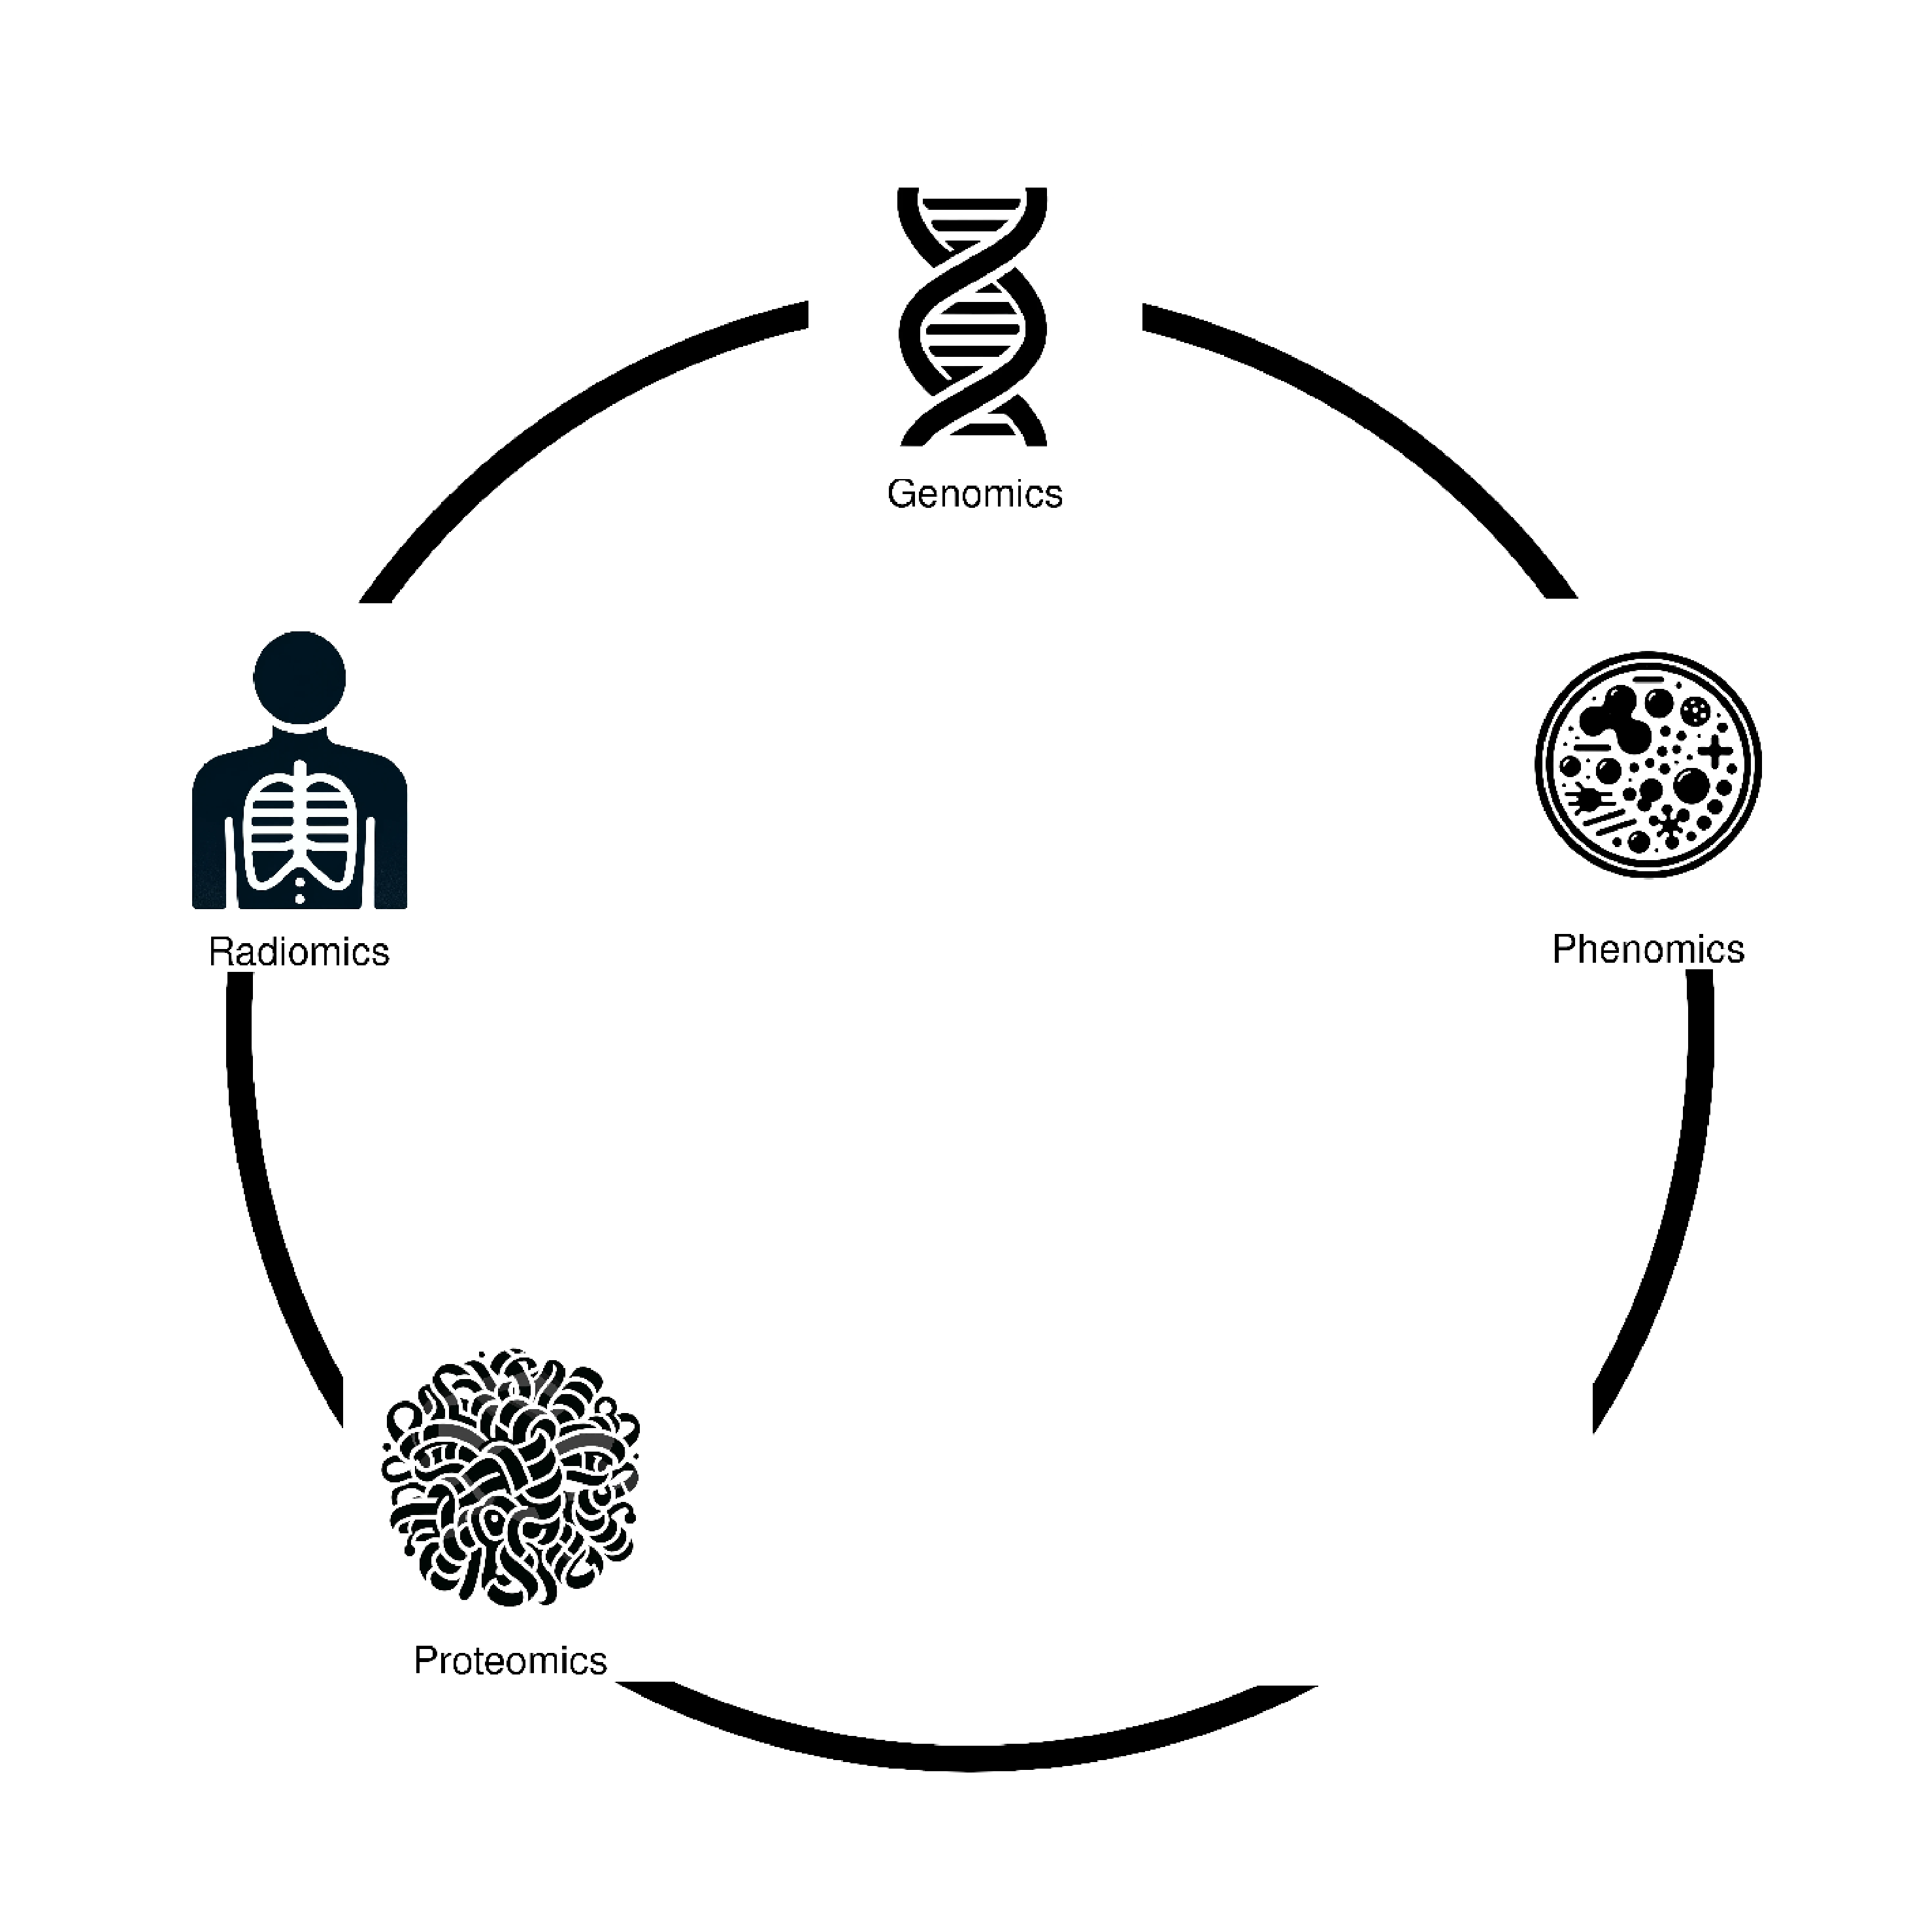
\includegraphics[width=\textwidth]{images/approaches_current.eps}
		\end{figure}
	\end{minipage} 
	\begin{minipage}{0.39\textwidth}
		\begin{block}{Personalised Medicine}
			characterizing a patient and customizing their treatment according to which sub-population they fall into	
		\end{block}
		\begin{block}{Problem}
			hard/risky/impossible to determine necessary biomarkers that would allow accurate diagnosis/treatment of disease
		\end{block}

	\end{minipage}
\end{frame}

\begin{frame}
	\frametitle{Towards Personalised Medicine: Future Approaches}
	\begin{minipage}{0.59\textwidth}
		\begin{figure}[H]
			\includegraphics[width=\textwidth]{images/approaches_future.eps}
		\end{figure}
	\end{minipage} \hfill
	\begin{minipage}{0.39\textwidth}
		\begin{block}{Model Based Approach}
			simulate clinically hard/ risky/ impossible to determine biomarkers that have a strong correlation with the disease outcome via first principles 
		\end{block}
		\begin{block}{Example}
			$\hookrightarrow$
		\end{block}
	\end{minipage}
\end{frame}
\begin{frame}
	\frametitle{Example: Bifurcation}
	\begin{figure}
	\begin{center}
		\begin{minipage}{0.43\linewidth}
		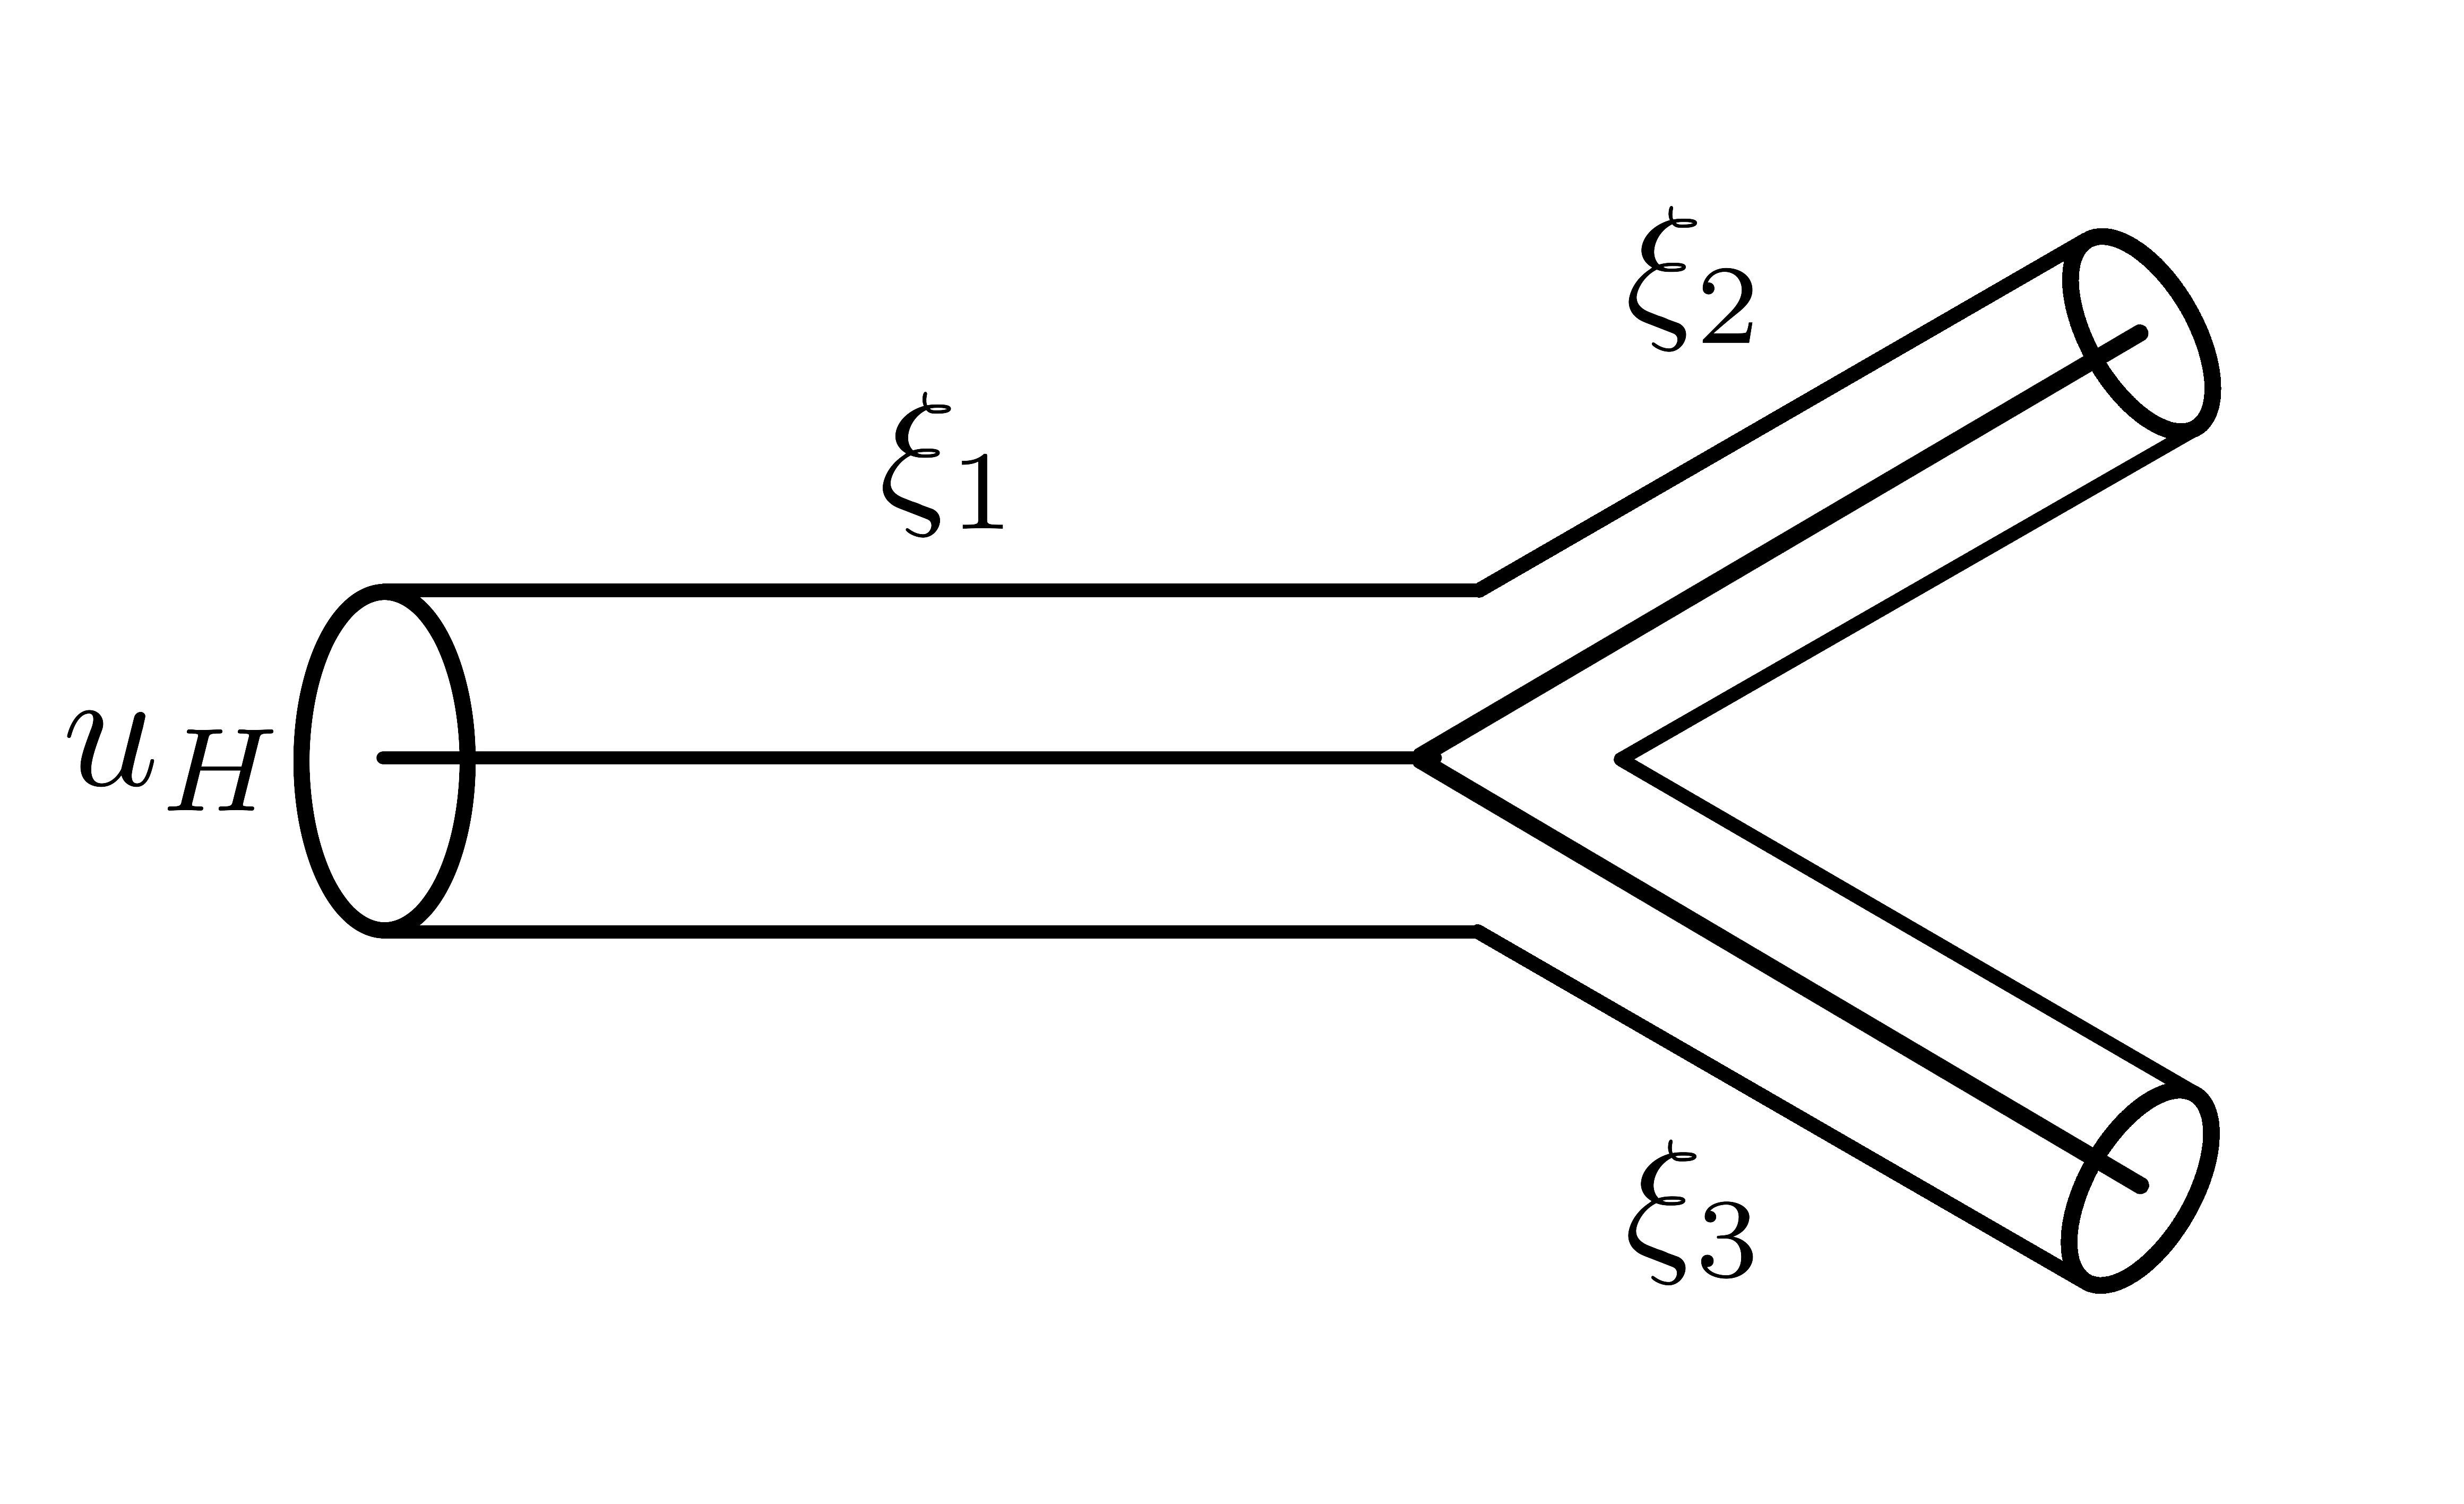
\includegraphics[width=\linewidth]{images/bifurcation.eps}
		\end{minipage}
		\hfill
		\begin{minipage}{0.1\linewidth}
		
\includegraphics[width=\linewidth]{images/right_arrow.png}
		\end{minipage}
		\hfill
		\begin{minipage}{0.43\linewidth}
		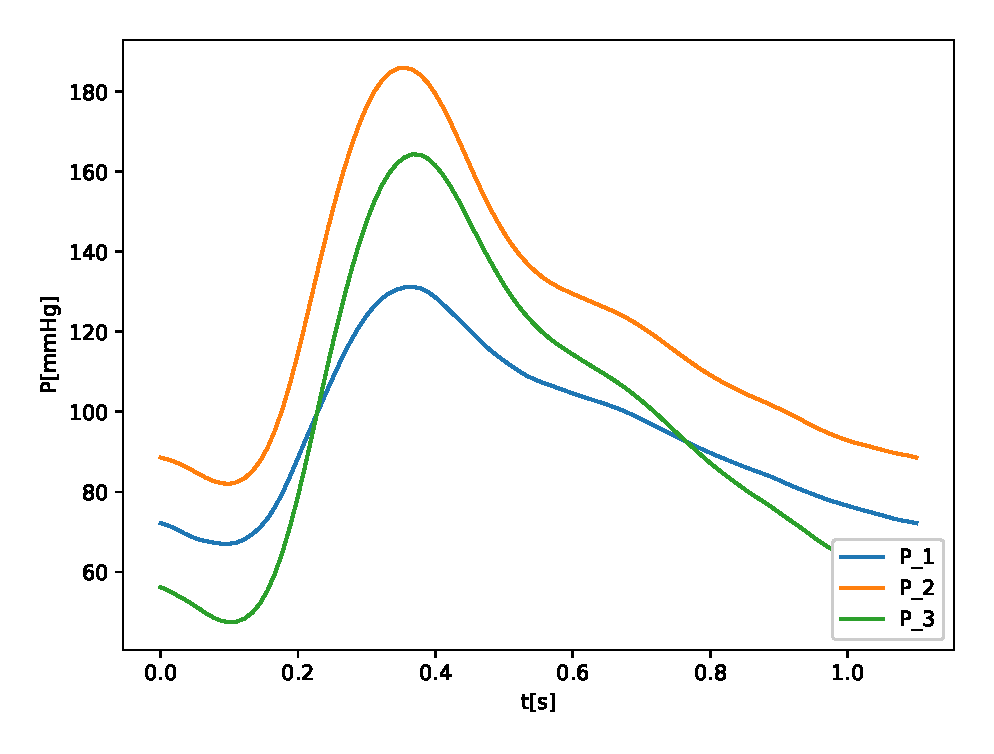
\includegraphics[width=\linewidth]{images/compare_output_params_P_P.eps}
		\end{minipage}
		%\begin{minipage}{0.48\linewidth}
		%	\captionof{figure}{test}
		%\end{minipage}
		%\hfill
		%\begin{minipage}{0.48\linewidth}
		%	\captionof{figure}{test}
		%\end{minipage}
		\begin{minipage}{0.43\linewidth}
			\caption*{The bifurcation $\xi := \{u_H, \xi_1, \xi_2, \xi_3\}$ consists of a driving flow $u_H$ and three vessels: $\xi_1 := \{l^1, h_0^1, A_0^1, E^1\}$, $\xi_2 := \{l^2, h_0^2, A_0^2, E^2, R_1^2, C^2, R_2^2\}$, $\xi_3 := \{l^3, h_0^3, A_0^3, E^3, R_1^3, C^3, R_2^3\}.$}
		\end{minipage}
		\hfill
		\begin{minipage}{0.43\linewidth}
			\caption*{Altering the Windkessel parameters $(R_1,C,R_2)$ leads to vastly different pressure waves being simulated.}
			\vfill
		\end{minipage}
	\end{center}
	\end{figure}
	{\tiny \centering 
		$u_H \hat{=}$ flow from heart,

		$l \hat{=}$ vessel length,
		$h_0 \hat{=}$ reference vessel wall thickness,
		$A_0 \hat{=}$ reference cross-section,

		$E \hat{=}$ Young's modulus,
		$R_1, C, R_2 \hat{=}$ Windkessel parameters.
	\par}
\end{frame}
\begin{frame}
	\frametitle{Example: Bifurcation}
	\begin{figure}
	\begin{center}
		\begin{minipage}{0.43\linewidth}
		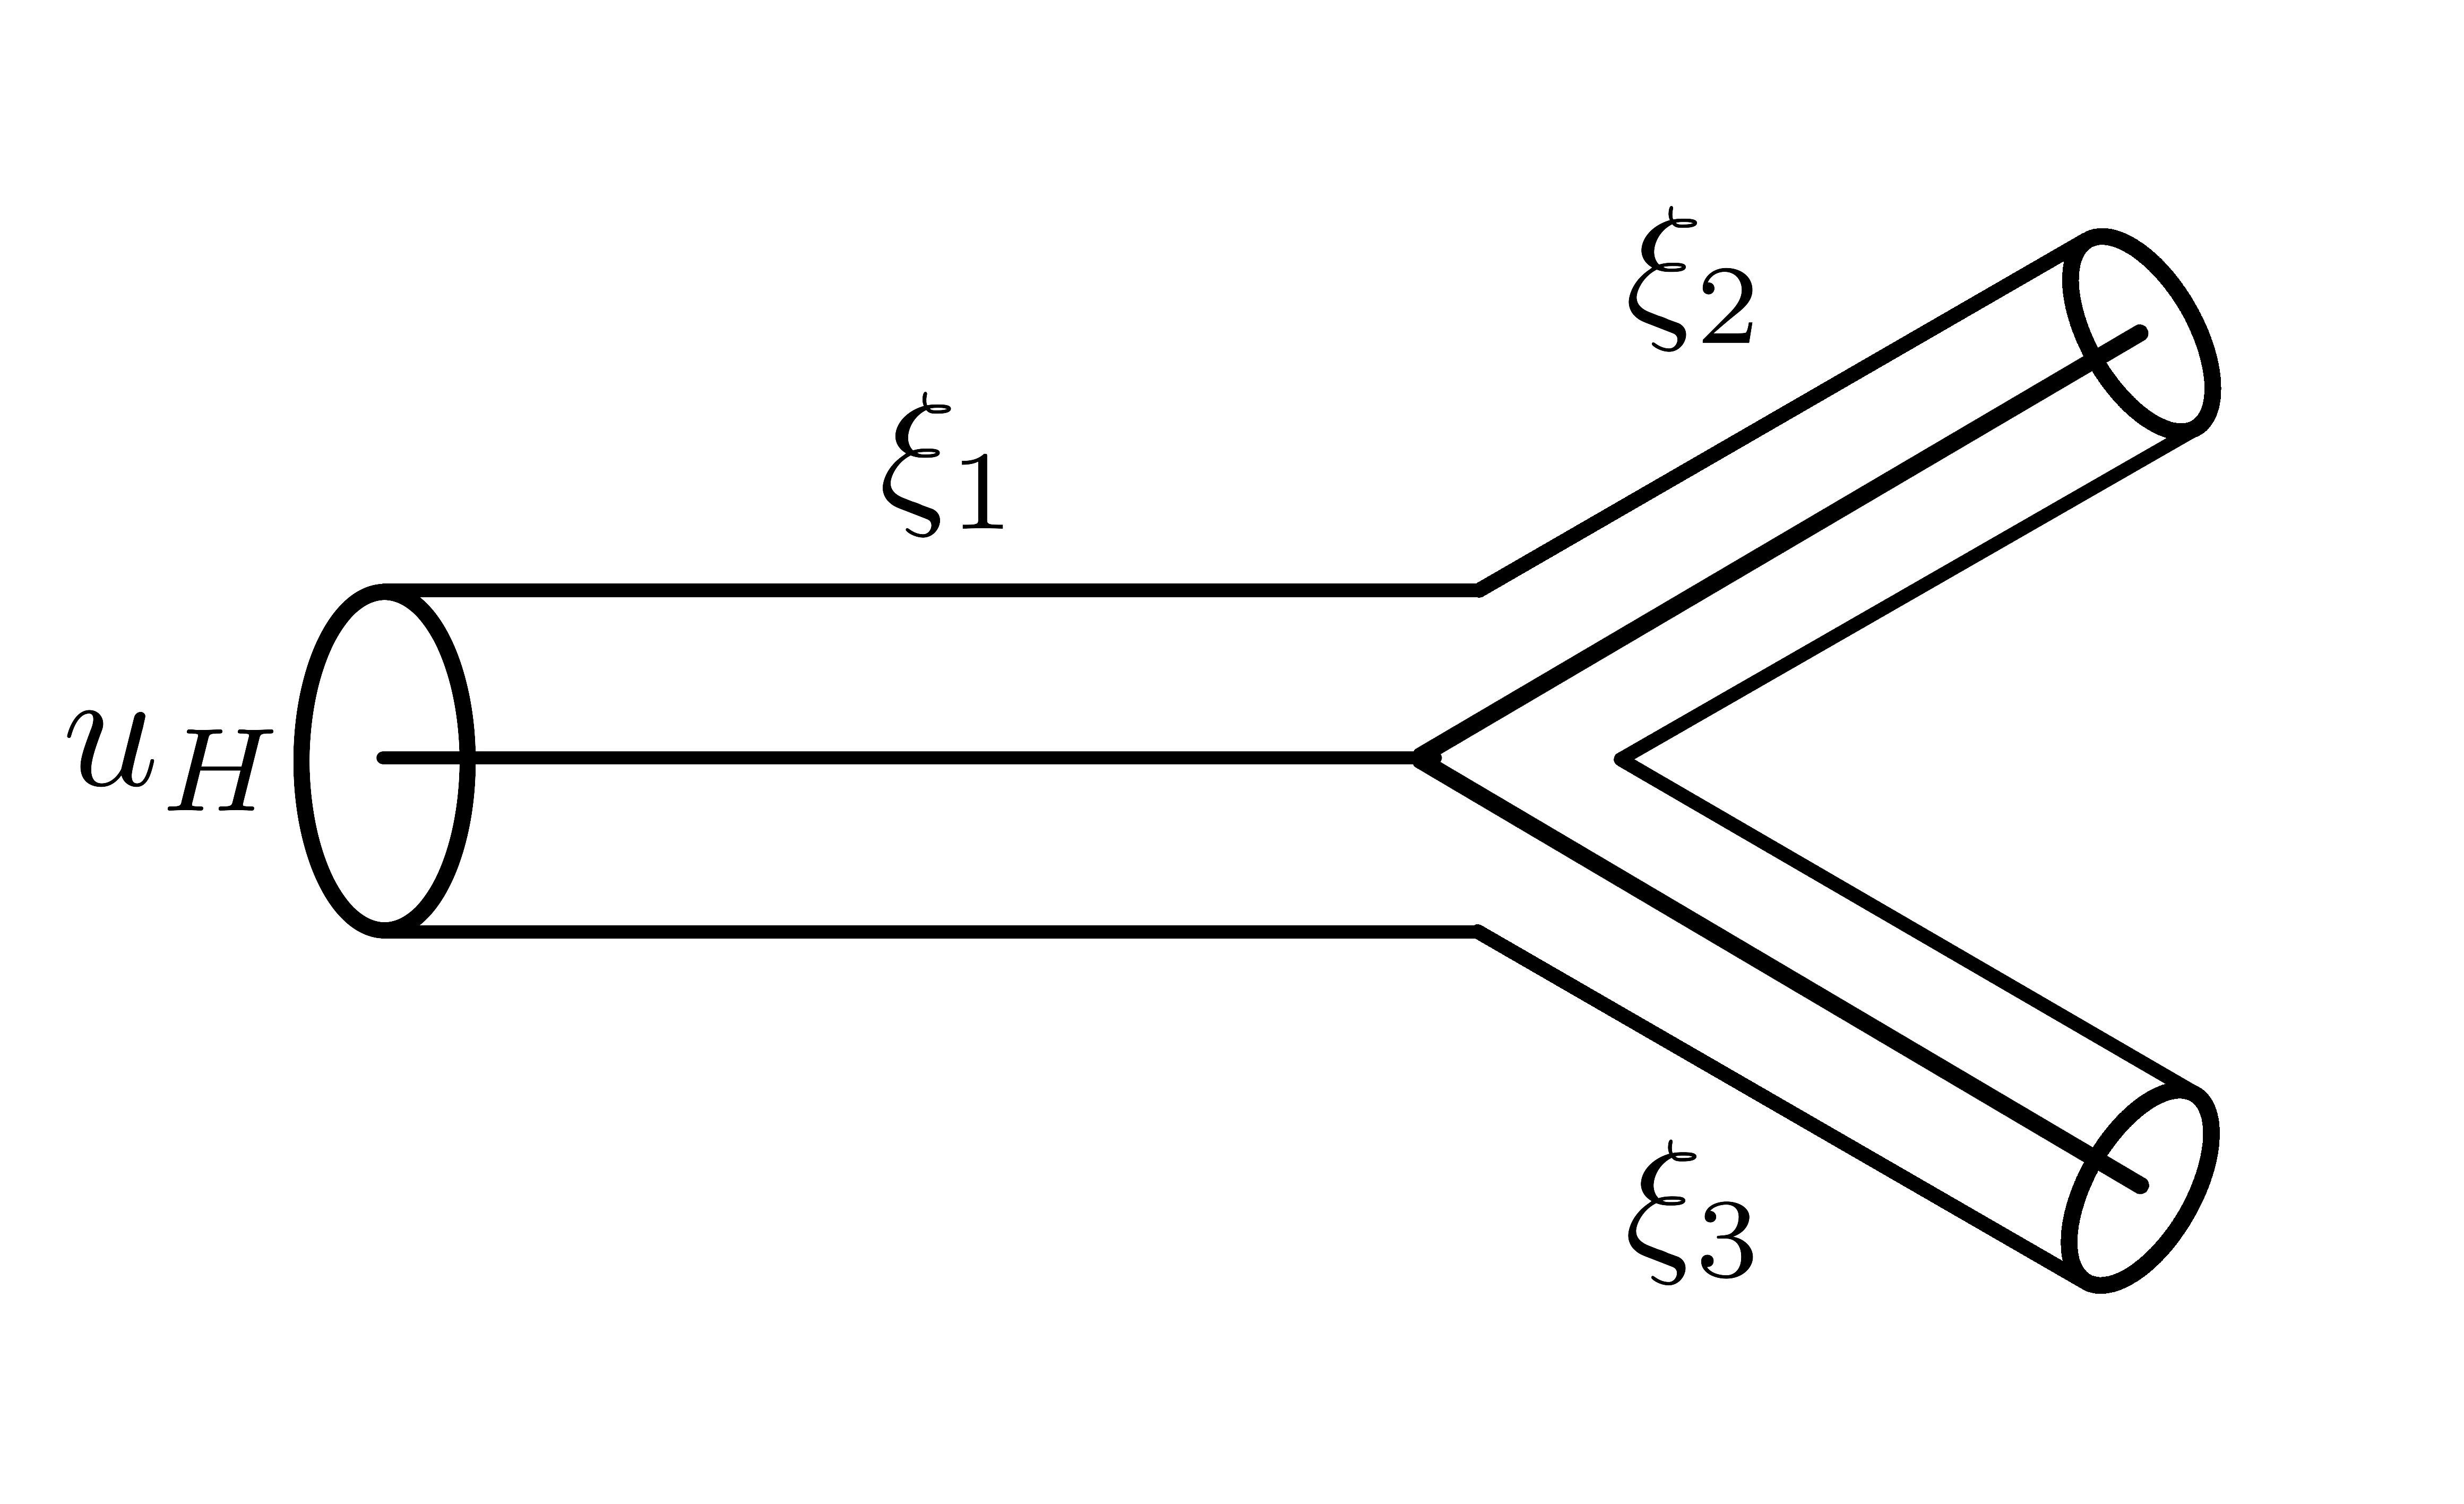
\includegraphics[width=\linewidth]{images/bifurcation.eps}
		\end{minipage}
		\hfill
		\begin{minipage}{0.1\linewidth}
		
\includegraphics[width=\linewidth]{images/right_arrow.png}
		\end{minipage}
		\hfill
		\begin{minipage}{0.43\linewidth}
		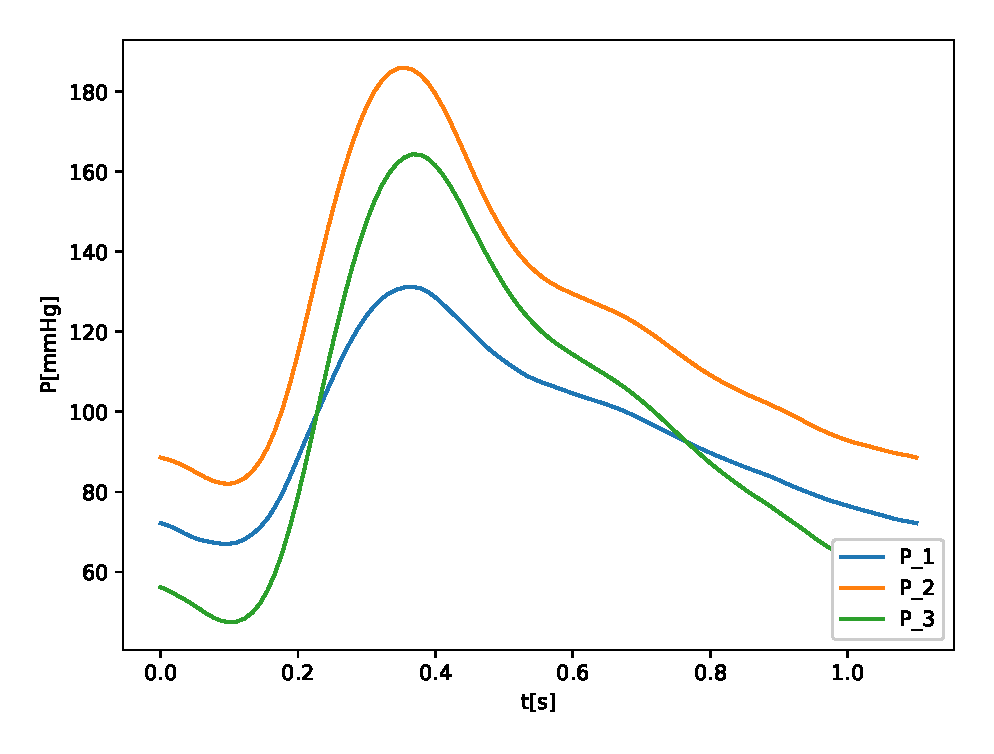
\includegraphics[width=\linewidth]{images/compare_output_params_P_P.eps}
		\end{minipage}
	\end{center}
	\end{figure}
		\begin{block}{Conclusion}
		The parameters are patient dependent and can heavily influence the simulation outcome. Therefore efficient methods of determining these parameters are necessary.
		\end{block}
\end{frame}

%\begin{frame}
%	\frametitle{Introduction}
%	\begin{block}{What is jaxFlowSim?}
%		\begin{itemize}
%			\item 1D-haemodynamics solver
%			\item written in JAX
%			\item differentiable
%		\end{itemize}
%	\end{block}
%	\vspace{5mm}
%\end{frame}

\begin{frame}
	\frametitle{3D Model Pipeline}

	$\vcenter{\hbox{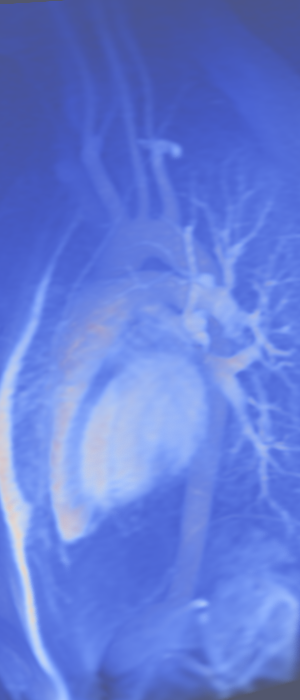
\includegraphics[width=0.2\textwidth]{images/medical_imaging_0007.eps}}}$
	$\vcenter{\hbox{
\includegraphics[width=0.1\textwidth]{images/right_arrow.png}}}$
	$\vcenter{\hbox{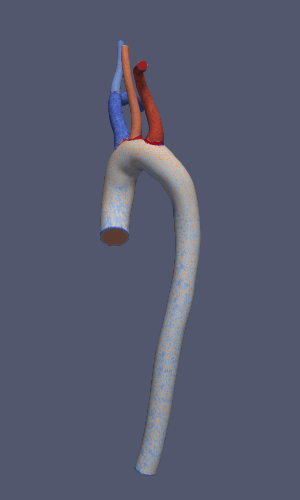
\includegraphics[width=0.2\textwidth]{images/3d_model_0007.eps}}}$
	$\vcenter{\hbox{
\includegraphics[width=0.1\textwidth]{images/right_arrow.png}}}$
	$\vcenter{\hbox{\includegraphics[width=0.2\textwidth]{images/1d_model_0007.eps}}}$
	$\vcenter{\hbox{
\includegraphics[width=0.1\textwidth]{images/right_arrow.png}}}$
	$\vcenter{\hbox{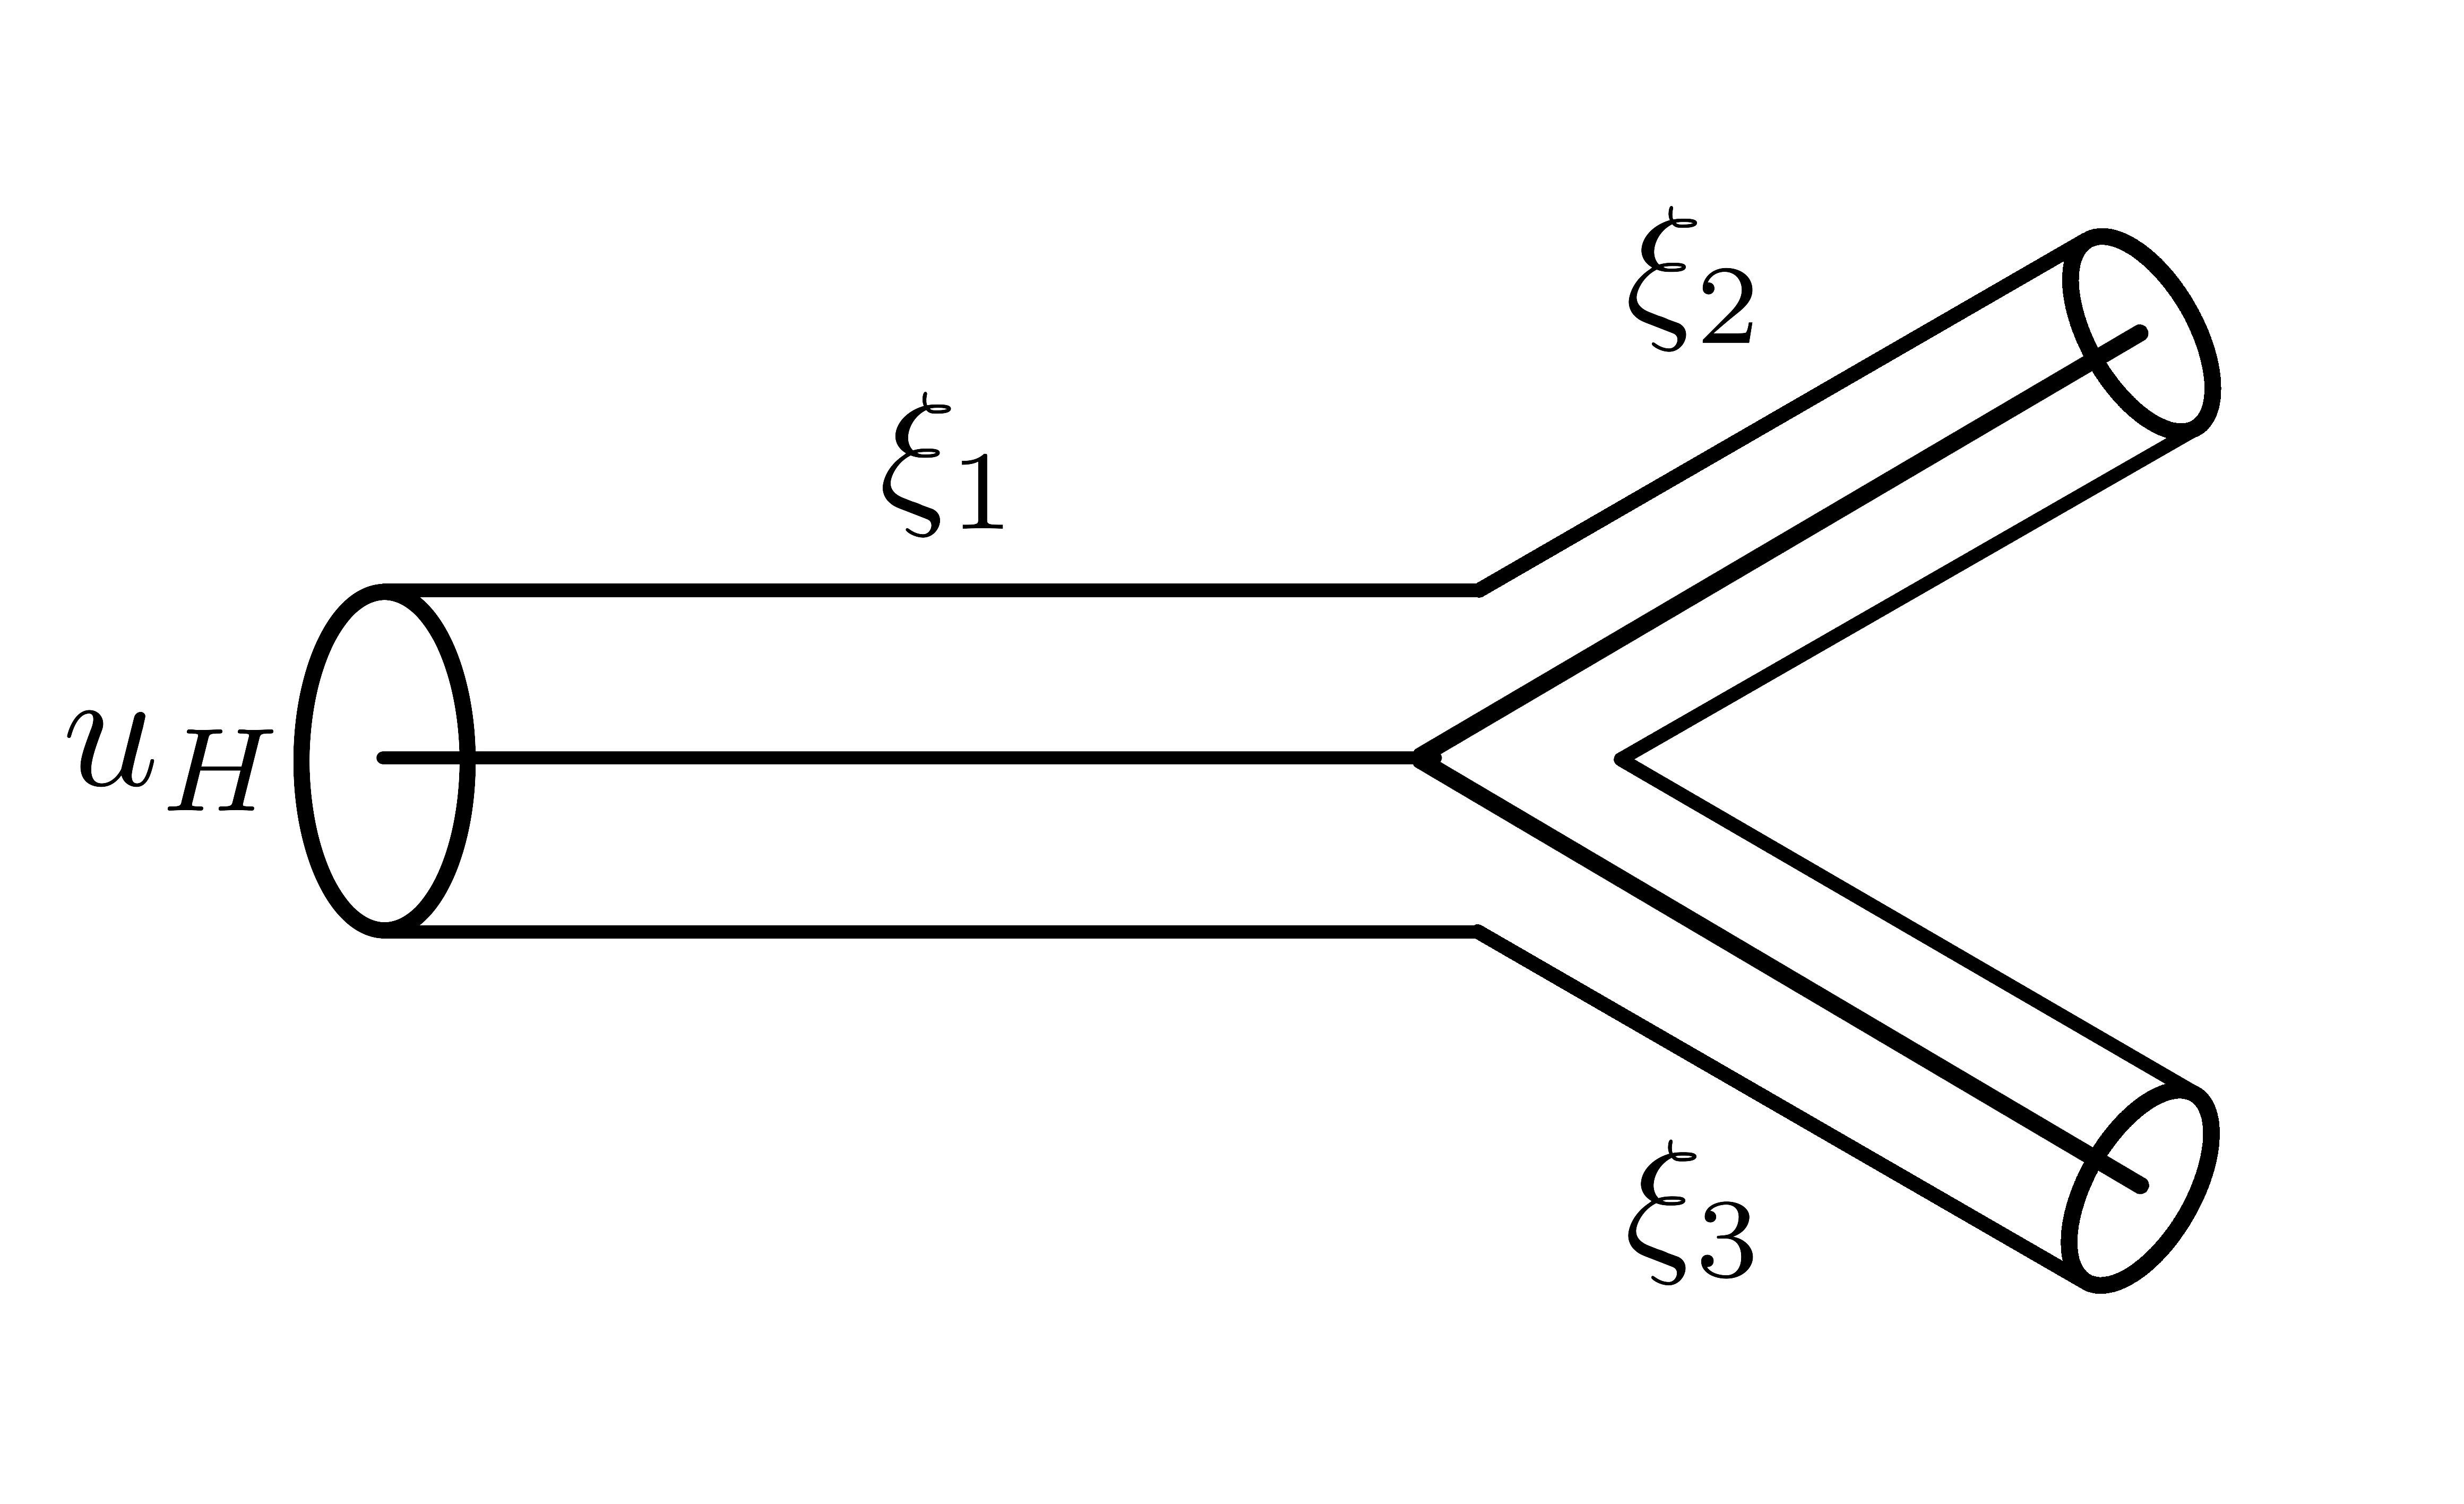
\includegraphics[width=0.2\textwidth]{images/bifurcation.eps}}}$
	$\vcenter{\hbox{
\includegraphics[width=0.1\textwidth]{images/right_arrow.png}}}$
	$\vcenter{\hbox{\includegraphics[width=0.2\textwidth]{images/3d_biomarkers_0007.eps}}}$
\end{frame}
%\begin{frame}
%	\frametitle{Motivation}
%	\begin{block}{Use and Novelty}
%		\begin{itemize}
%			\item towards personalised medicine
%			\item parameter inference
%			\item sensitivity analysis
%		\end{itemize}
%	\end{block}
%	\vspace{5mm}
%\end{frame}

\section{Model}

\begin{frame}
	\frametitle{1D-Navier Stokes Equations}
	\begin{equation}
		\begin{aligned}
			\frac{\partial \mathbf{U}}{\partial t} + \frac{\partial \mathbf{F} \left(
			\mathbf{U} \right)}{\partial z} &= \mathbf{S} \left( \mathbf{U} \right), \ t>0, \
			z \in \left[ 0,l \right], \\
			\mathbf{U} \left( z;0 \right) &= \mathbf{U}_0 \left( z \right), \ z \in \left[ 0,l \right], \\
			\mathbf{U} \left( 0;t \right) &= \mathbf{U}_L \left( t \right), \ t>0,\\
			\mathbf{U} \left( l;t \right) &= \mathbf{U}_R \left( t \right), \ t>0,
		\end{aligned} \label{eq:1deqs3}
	\end{equation}
	\begin{equation}
		\mathbf{U} :=
		\begin{bmatrix}
			A \\
			Q
		\end{bmatrix}, \ 
		\mathbf{F} \left( \mathbf{U} \right) :=
		\begin{bmatrix}
			Q \\
			\frac{Q^2}{A} + \frac{\beta A^{\frac{3}{2}}}{3\rho\sqrt{A_0}}
		\end{bmatrix}, \ 
		\mathbf{S} \left( \mathbf{U} \right) :=
		\begin{bmatrix}
			0 \\
			-22\frac{\mu}{\rho}\frac{Q}{A}
		\end{bmatrix}.
	\end{equation}

	\vfill

	{\tiny \centering 
		$\mathbf{U_0} \hat{=}$ initial condition, 
		$\mathbf{U_L} \hat{=}$ left boundary values,
		$\mathbf{U_R} \hat{=}$ right boundary values,

		$l \hat{=}$ vessel length,
		$A \hat{=}$ cross-section,
		$A_0 \hat{=}$ reference cross-section,
		$Q \hat{=}$ volumetric flow-rate,

		$\beta \hat{=}$ elasticity coefficient,
		$\rho \hat{=}$ blood density,
		$\mu \hat{=}$ blood dynamic viscosity. 
	\par}


\end{frame}

\begin{frame}
	\frametitle{Tube Law}
	\begin{align}
		P(z;t) &:= P_{ext}(z;t) + \beta \left( \sqrt{\frac{A(z;t)}{A_0(z)}}-1 \right),      \label{eq:p_tot}\\
		\beta(z) &:=  \frac{\sqrt{\pi} E h_0(z)}{(1-\nu^2) \sqrt{A_0(z)}},\  z \in \left[ 0,l \right], \ t > 0. 
	\end{align}

	\vfill

	{\tiny \centering 
		$P \hat{=}$ pressure,
		$P_{ext} \hat{=}$ external pressure,

		$l \hat{=}$ vessel length,
		$A \hat{=}$ cross-section,
		$A_0 \hat{=}$ reference cross-section,

		$E \hat{=}$ Young's modulus,
		$h_0 \hat{=}$ reference vessel wall thickness,
		$\nu \hat{=}$ Poisson's ratio (elasticity parameter). 
	\par}

\end{frame}

\begin{frame}
	\frametitle{Initial Conditions}
	\begin{align}
		u(z;0) &\equiv 0, &z \in [0,l],\\
		A(z;0) &= A_0(z), &z \in [0,l], \\
		Q(z;0) &= u(z;0)A(z;0) \equiv 0, &z \in [0,l].
	\end{align}
	\vspace{5mm}
\end{frame}
\begin{frame}
	\frametitle{Inlets, Juntions, Outlets}
	\begin{block}{Inlets}
		set $P$ from data $\rightarrow$ set $u$, $Q$, $A$, $c$ through linear extrapolation of charateristics

		set $Q$ from data $\rightarrow$ set $u$, $A$, $c$, $P$ through linear extrapolation of charateristics
	\end{block}
	\begin{block}{Junctions}
		solve linear system of equations consisting of:
		\begin{itemize}
			\item conservation of mass, 
			\item conservation of pressure, 
			\item extrapolation of charateristics	
		\end{itemize}
	\end{block}
	\begin{block}{Outlets}
		0D-/ lumped parameter model: three element Windkessel (RCR) model 
	\end{block}
\end{frame}
\begin{frame}
	\frametitle{Numerical Methods}
	\begin{block}{1D-Model}
		FV method: MUSCL scheme with Lax-Friedrichs Flux
	\end{block}
	\begin{block}{Junctions \& Outlets}
		Newton method
	\end{block}


\end{frame}

\section{Implementation}

\begin{frame} [fragile]
	\frametitle{Code Structure}
	\begin{lstlisting}[basicstyle=\fontsize{7}{7}\selectfont\ttfamily, language=Python, caption={$dt \hat{=}$timestep(CFL), setBoundaryValues$\hat{=}$inlet(from data), outlet(Windkessel),junctions(conservation laws), muscl$\hat{=}$Monotonic Upstream-centered Scheme for Conservation Laws(Finite Volume)}, label=lst:pc, escapechar=|] 
		def runSimulation(config_filename, J) 
			config = loadConfig(config_filename) |\label{ln:init_start}|
			simulation_data = buildArterialNetwork(config) |\label{ln:init_end}|

			P_t = [0] |\label{ln:pt}|

			converged = False |\label{ln:whout1}|
			while not converged: |\label{ln:whout2}|
				t = 0 |\label{ln:t0}|
				i = 0 |\label{ln:i0}|
				P_t_temp = P_t |\label{ln:cp}|
				while t < T:
					dt = computeDt(simulation_data) |\label{ln:cfl}|
					simulation_data = setBoundaryValues(simulation_data, dt) |\label{ln:bv    }|
					simulation_data = muscl(simulation_data, dt) |\label{ln:muscl}|
					P_t[i,:] = savePressure(simulation_data) |\label{ln:svp}|
					t = t + dt |\label{ln:updt}|
				i = i + 1 |\label{ln:updi}|
				if i >= J:
					break
				converged = checkConv(P_t, P_t_temp) |\label{ln:conv}|
\end{lstlisting}
\end{frame}
\begin{frame}
	\frametitle{Padding}
	without padding
	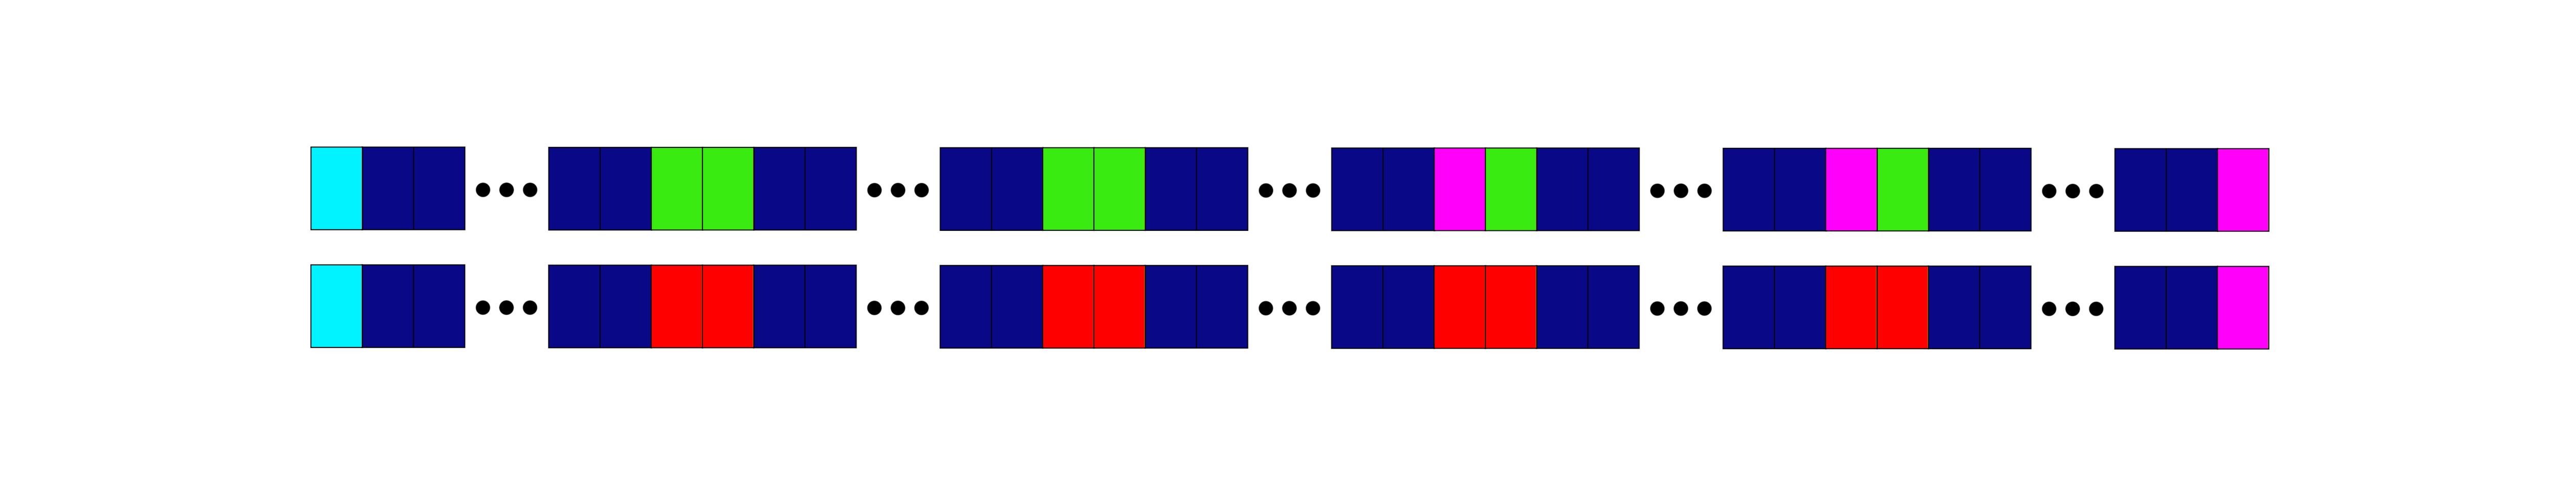
\includegraphics[width=\textwidth]{images/padding1.eps}
	with padding
	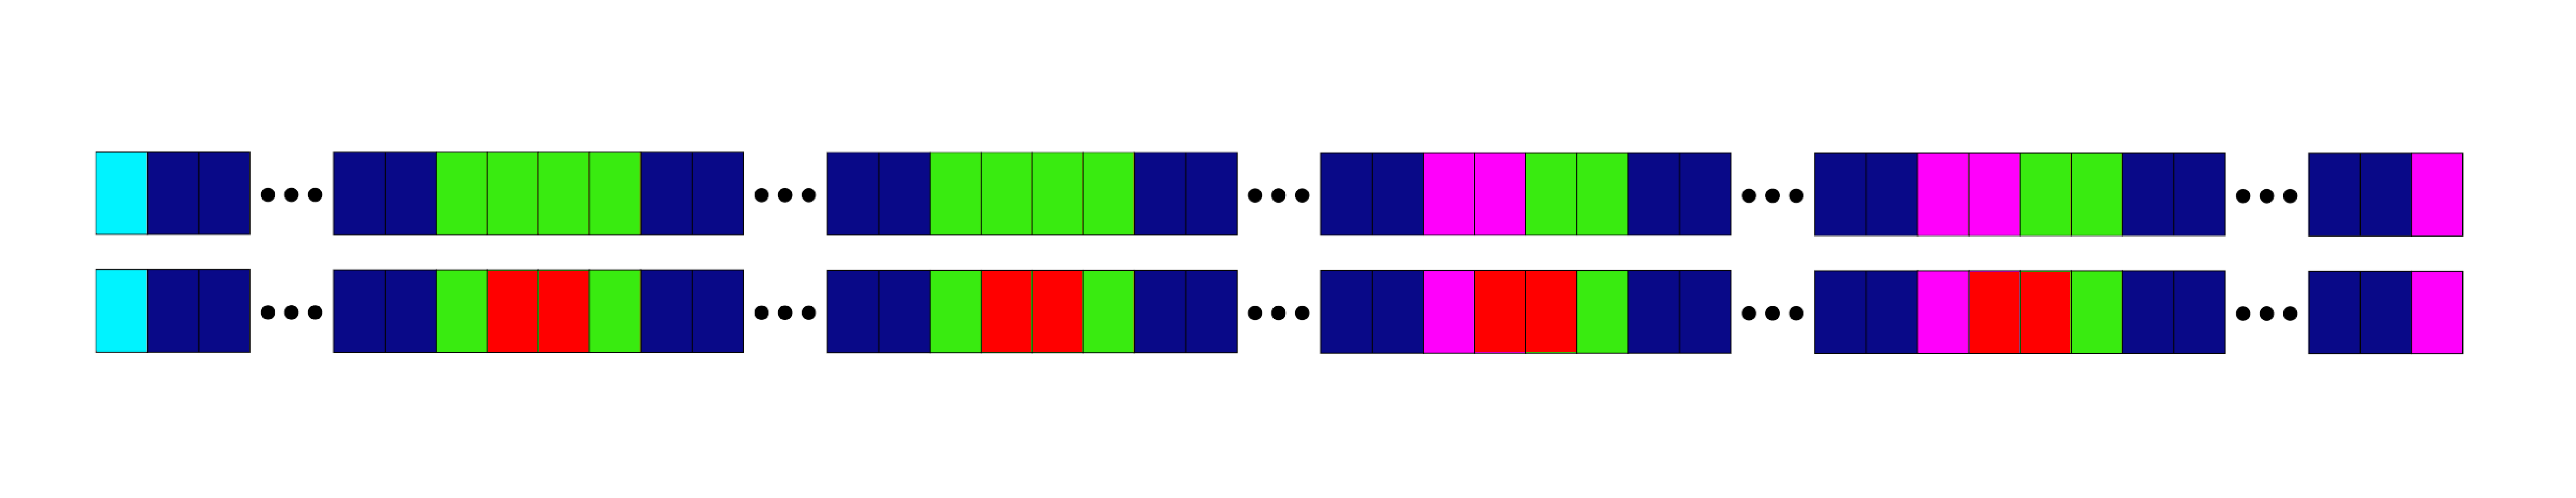
\includegraphics[width=\textwidth]{images/padding2.eps}
	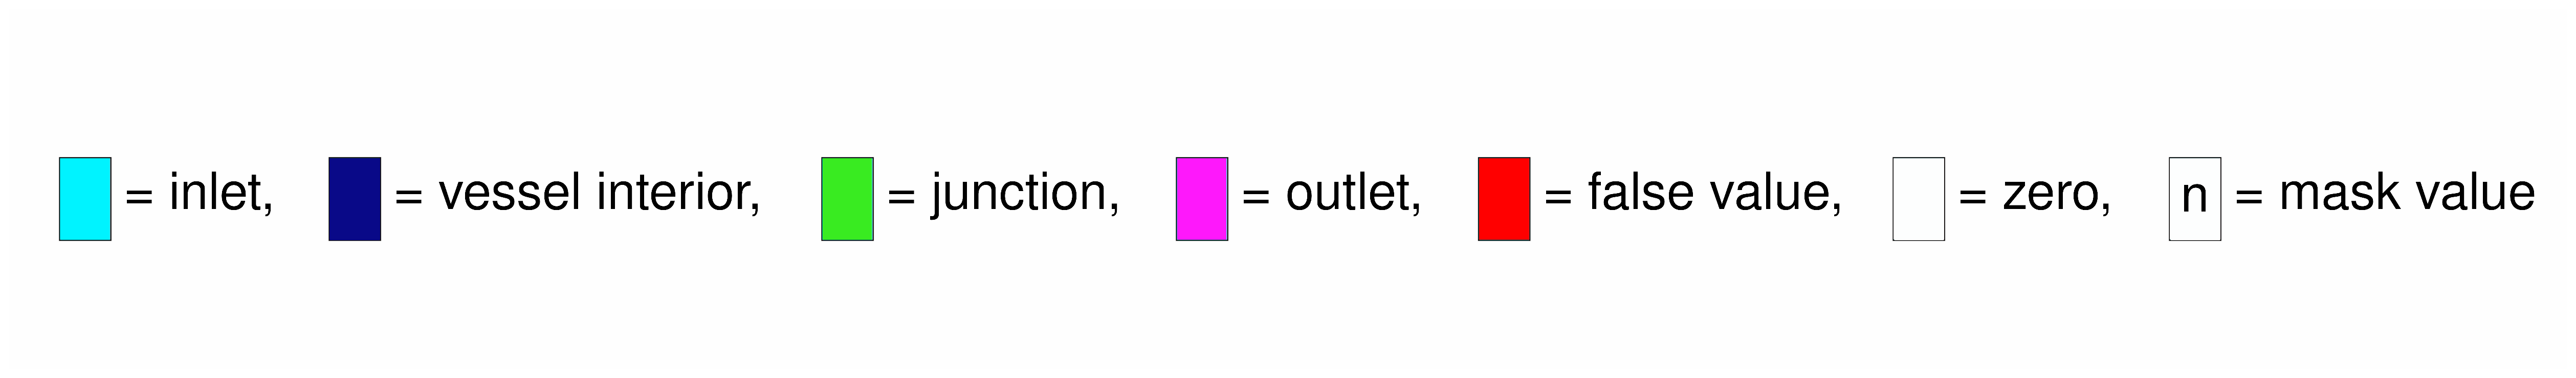
\includegraphics[width=\textwidth]{images/legend.eps}
\end{frame}
\begin{frame}
	\frametitle{Masking}
	\includegraphics[width=\textwidth]{images/masking.eps}
	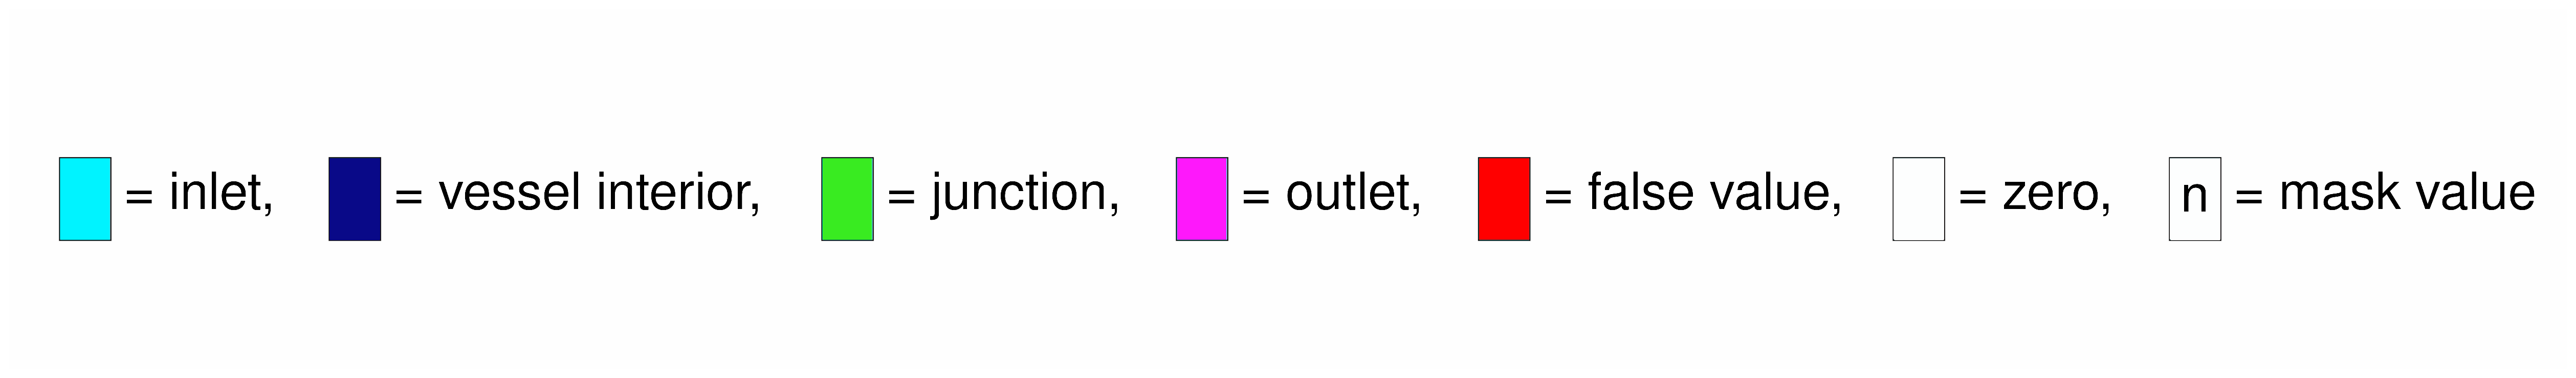
\includegraphics[width=\textwidth]{images/legend.eps}
\end{frame}

\section{Results}
\begin{frame}
	\frametitle{Model: Aorta (0007\_H\_AO\_H)}
	\begin{figure} [H]
		\centering
		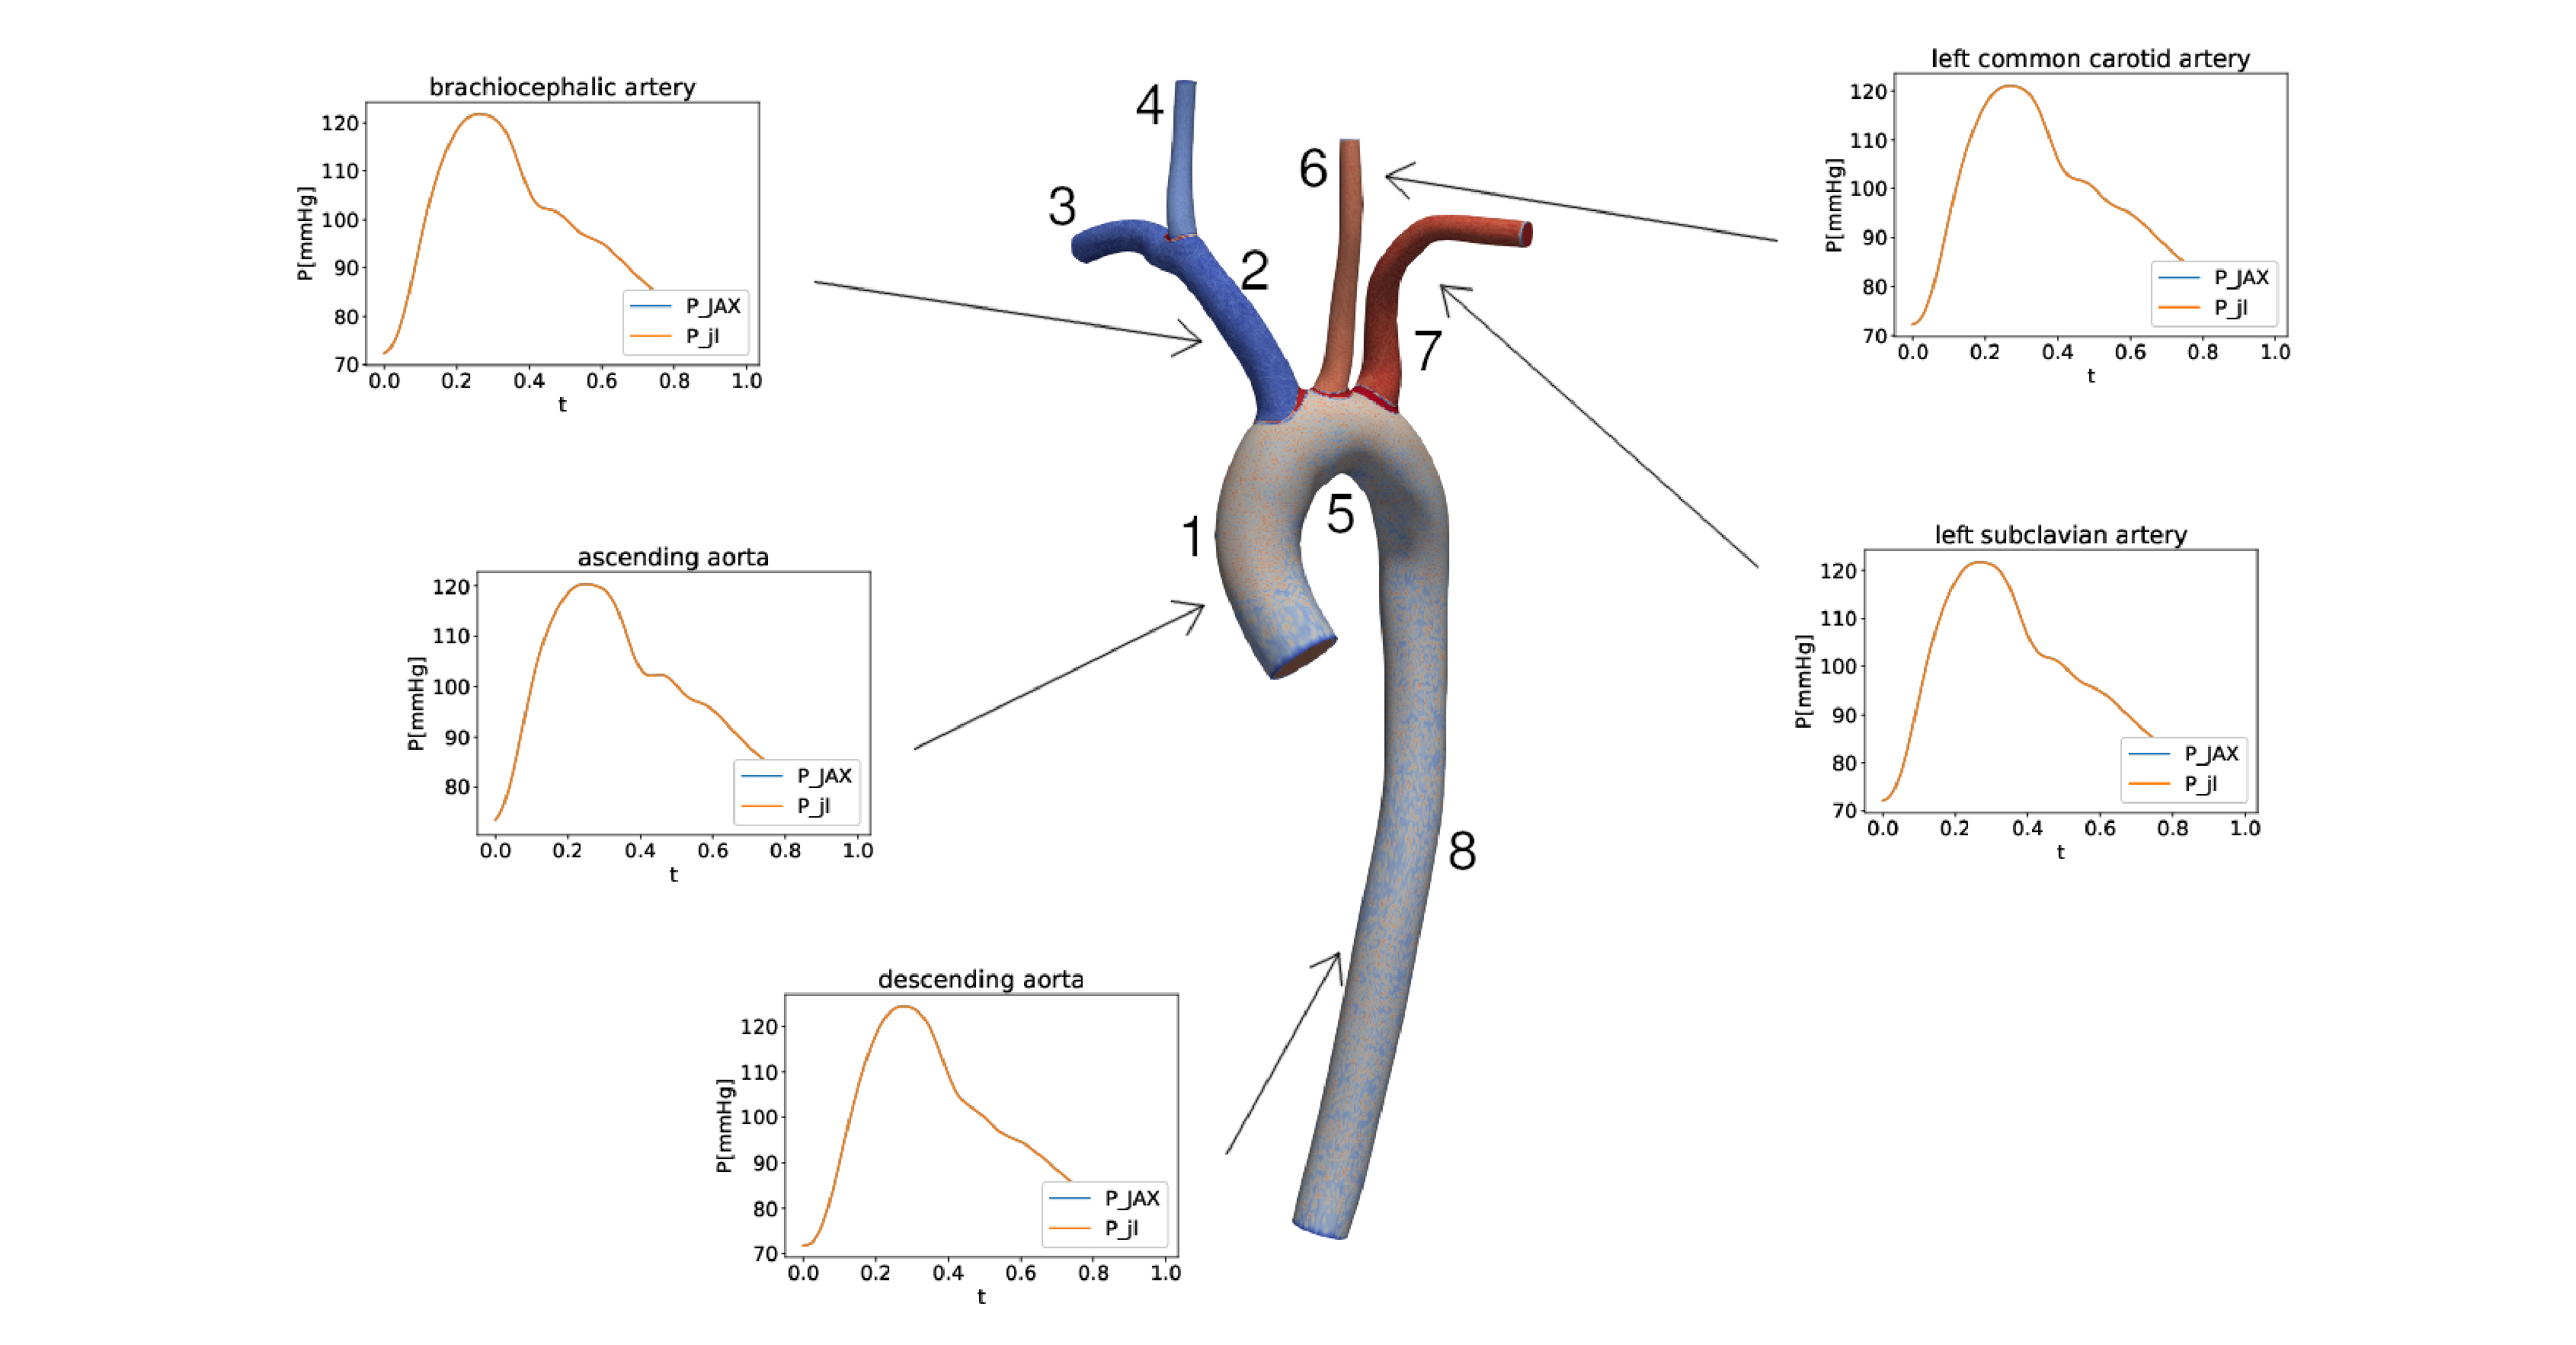
\includegraphics[width=\columnwidth]{images/0007.eps}
		\label{fig:aorta}
	\end{figure}
\end{frame}
\begin{frame}
	\frametitle{Model: Abdominal Arteries (0029\_H\_ABAO\_H)}
	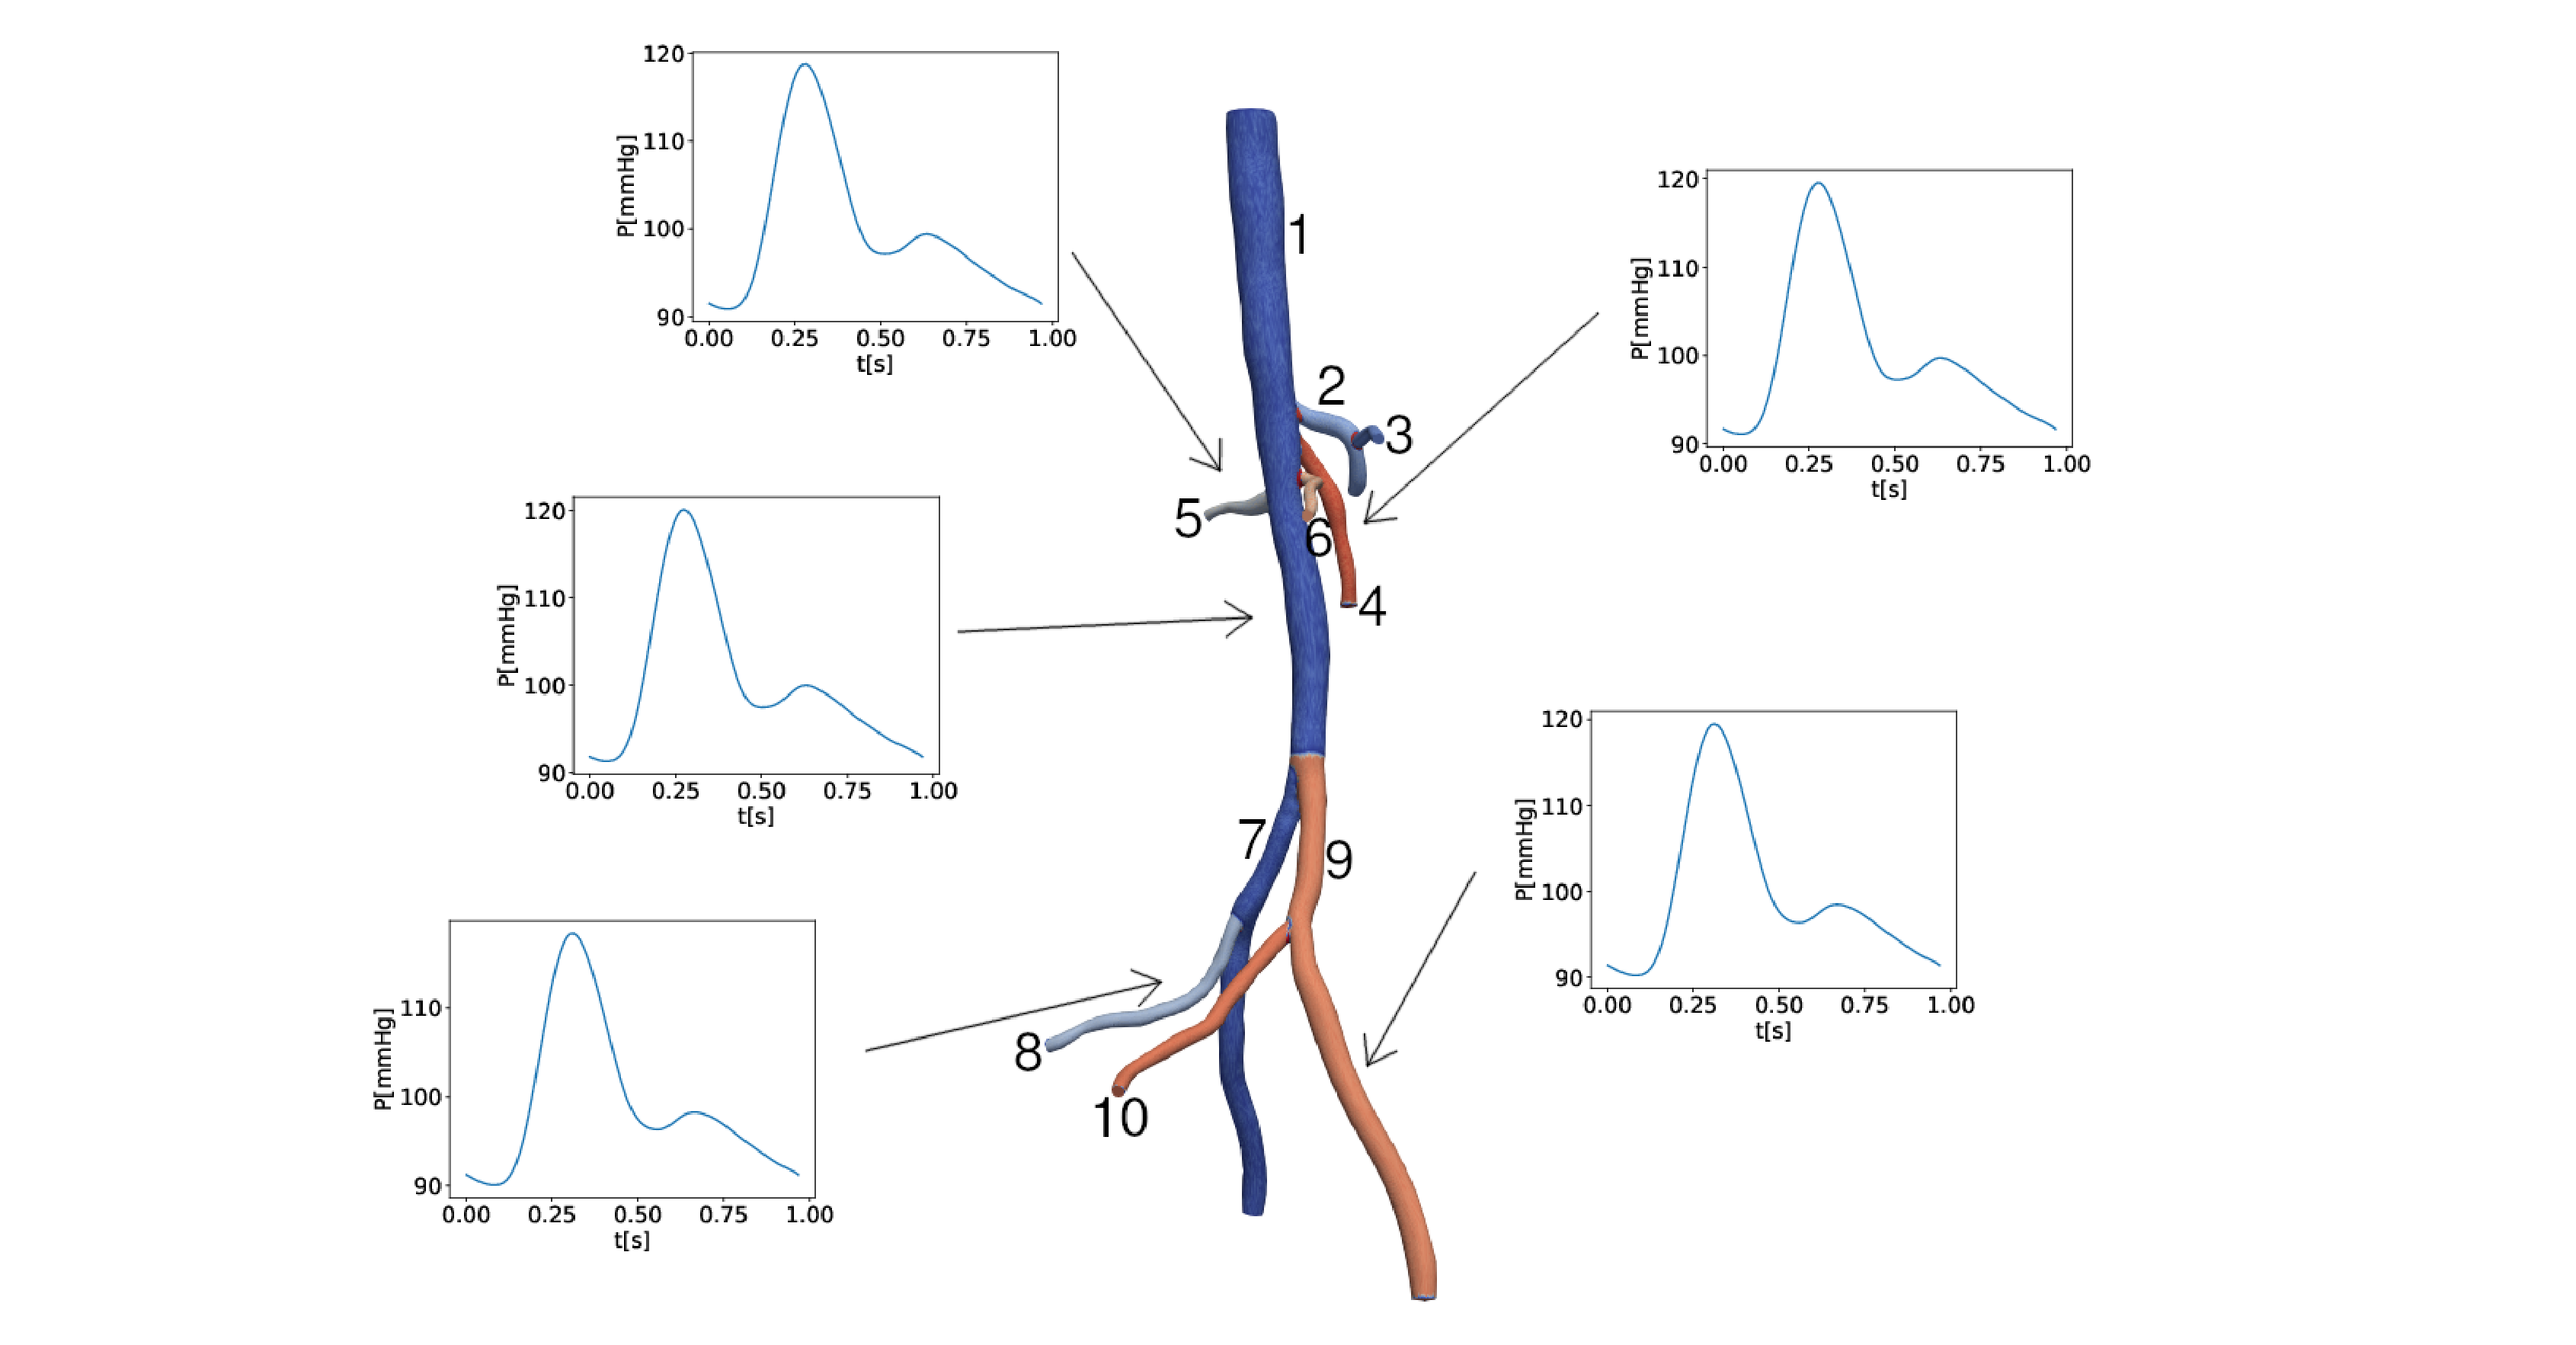
\includegraphics[width=\columnwidth]{images/0029.eps}
\end{frame}
\begin{frame}
	\frametitle{Model: Cerebellar Arteries (0053\_H\_CERE\_H)}
	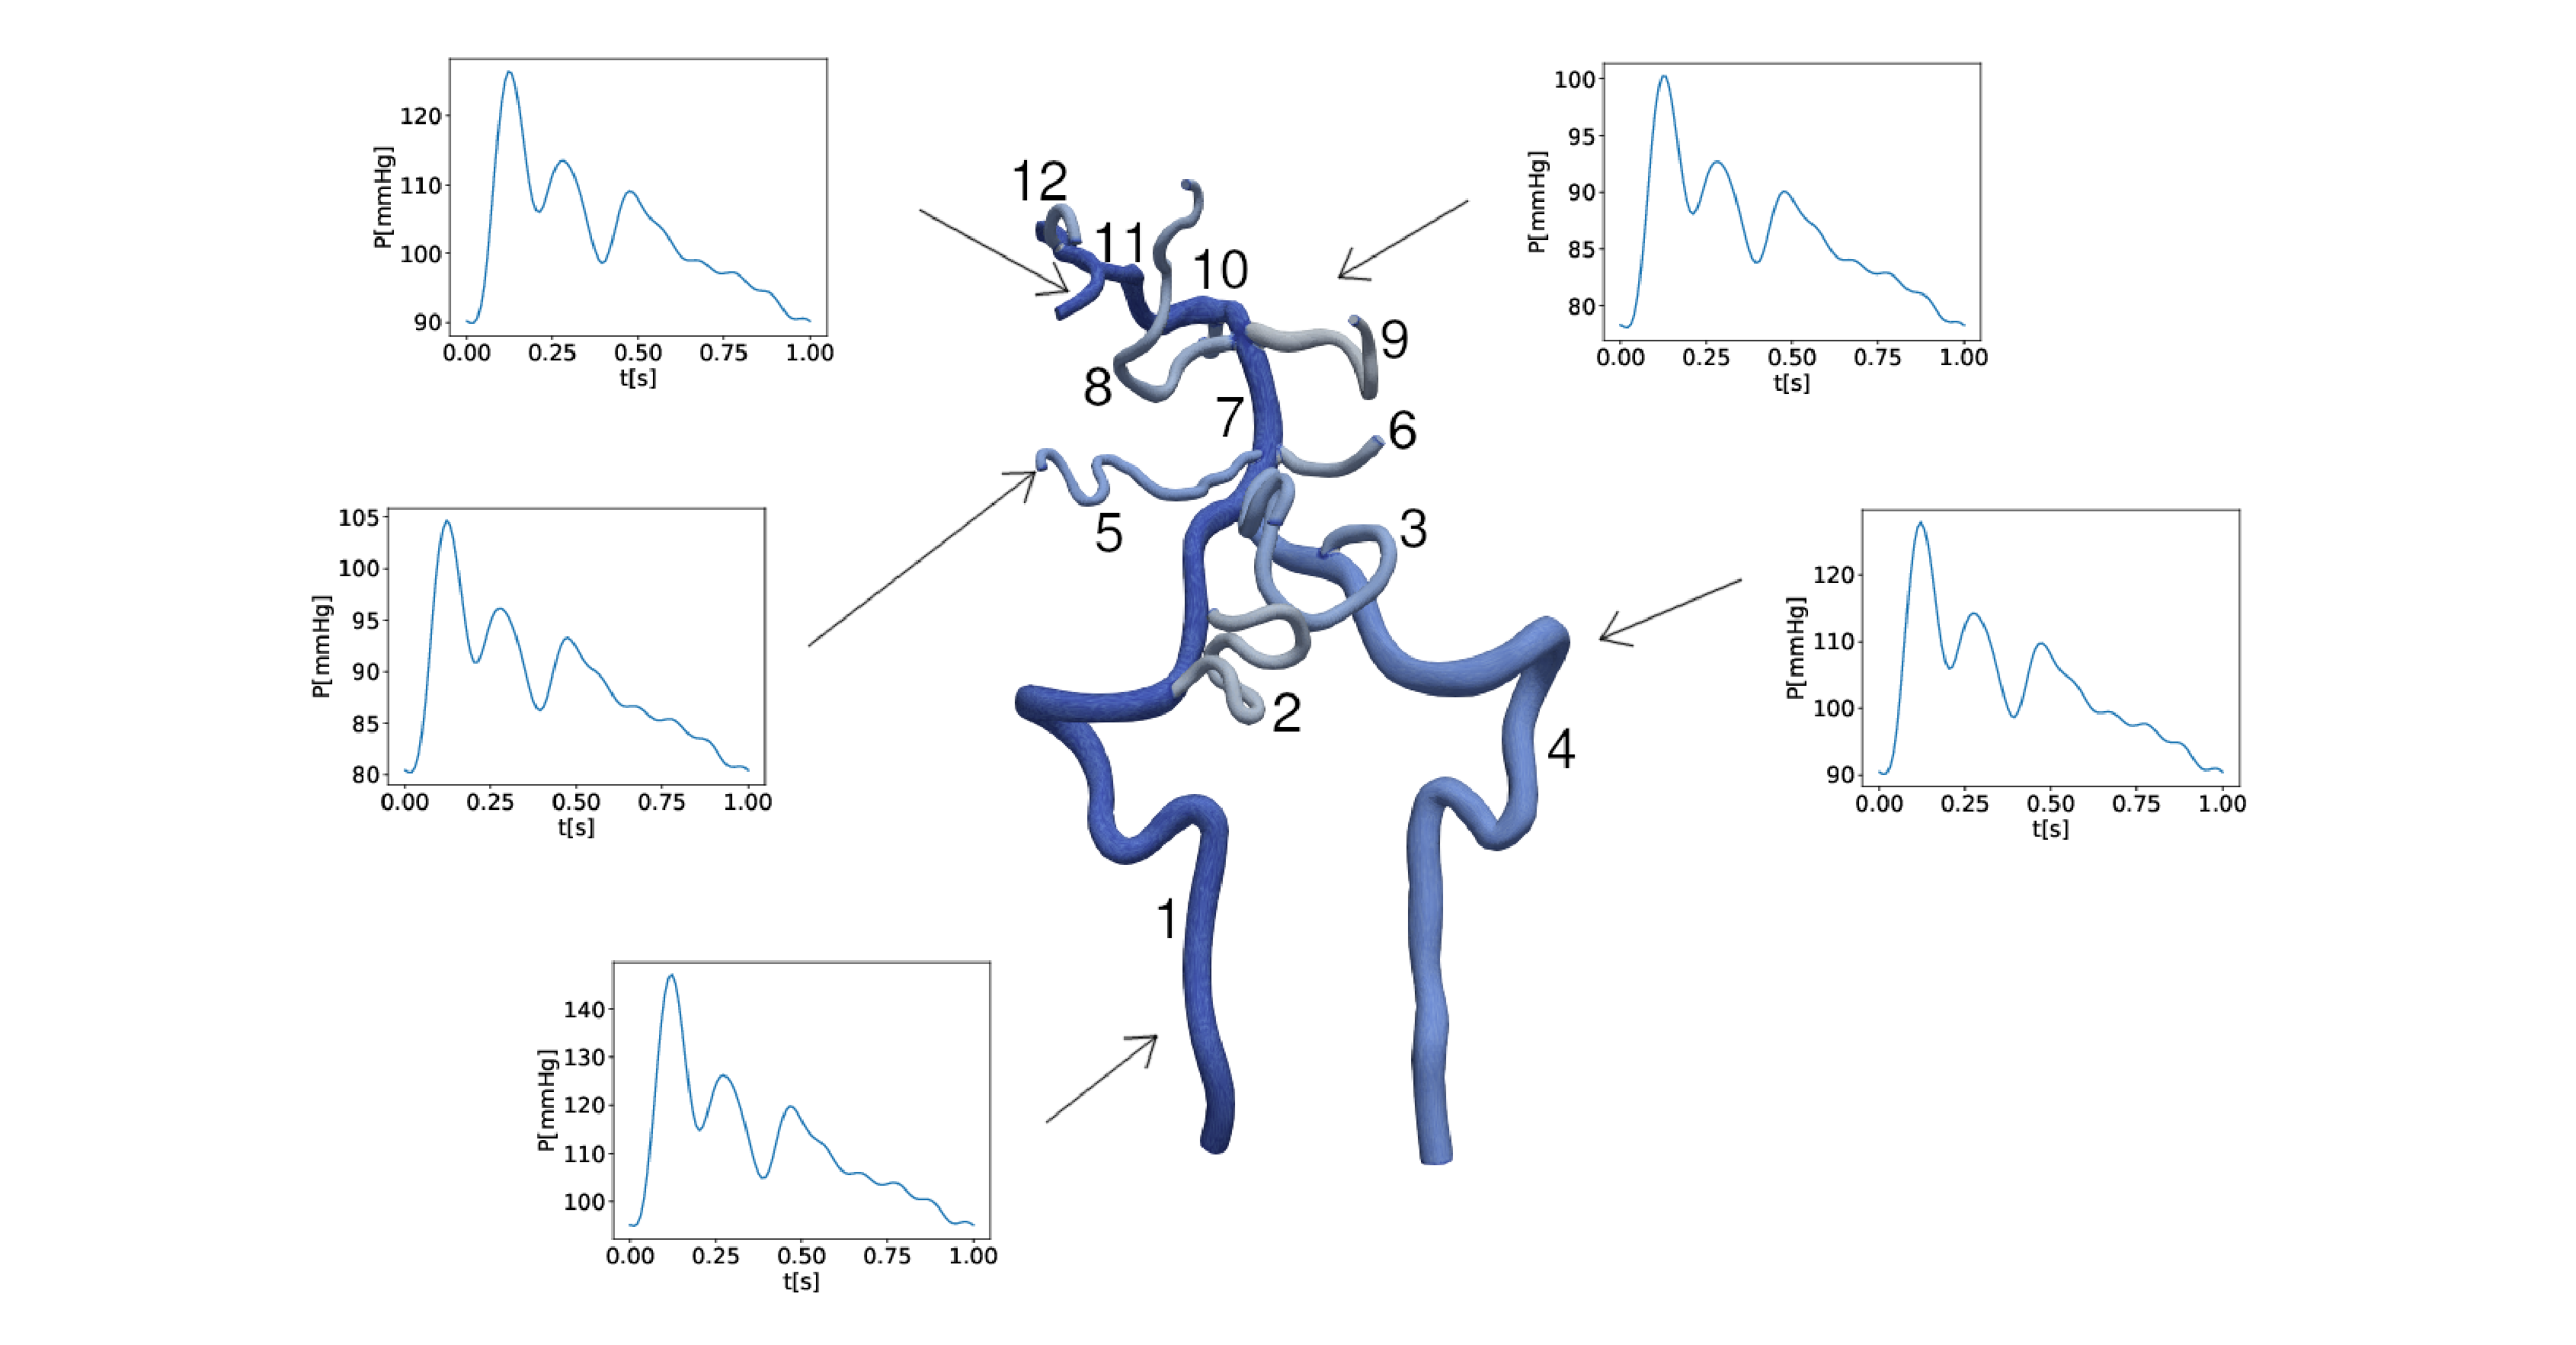
\includegraphics[width=\columnwidth]{images/0053.eps}
\end{frame}
\begin{frame}
	\frametitle{Model: ADAN56}
	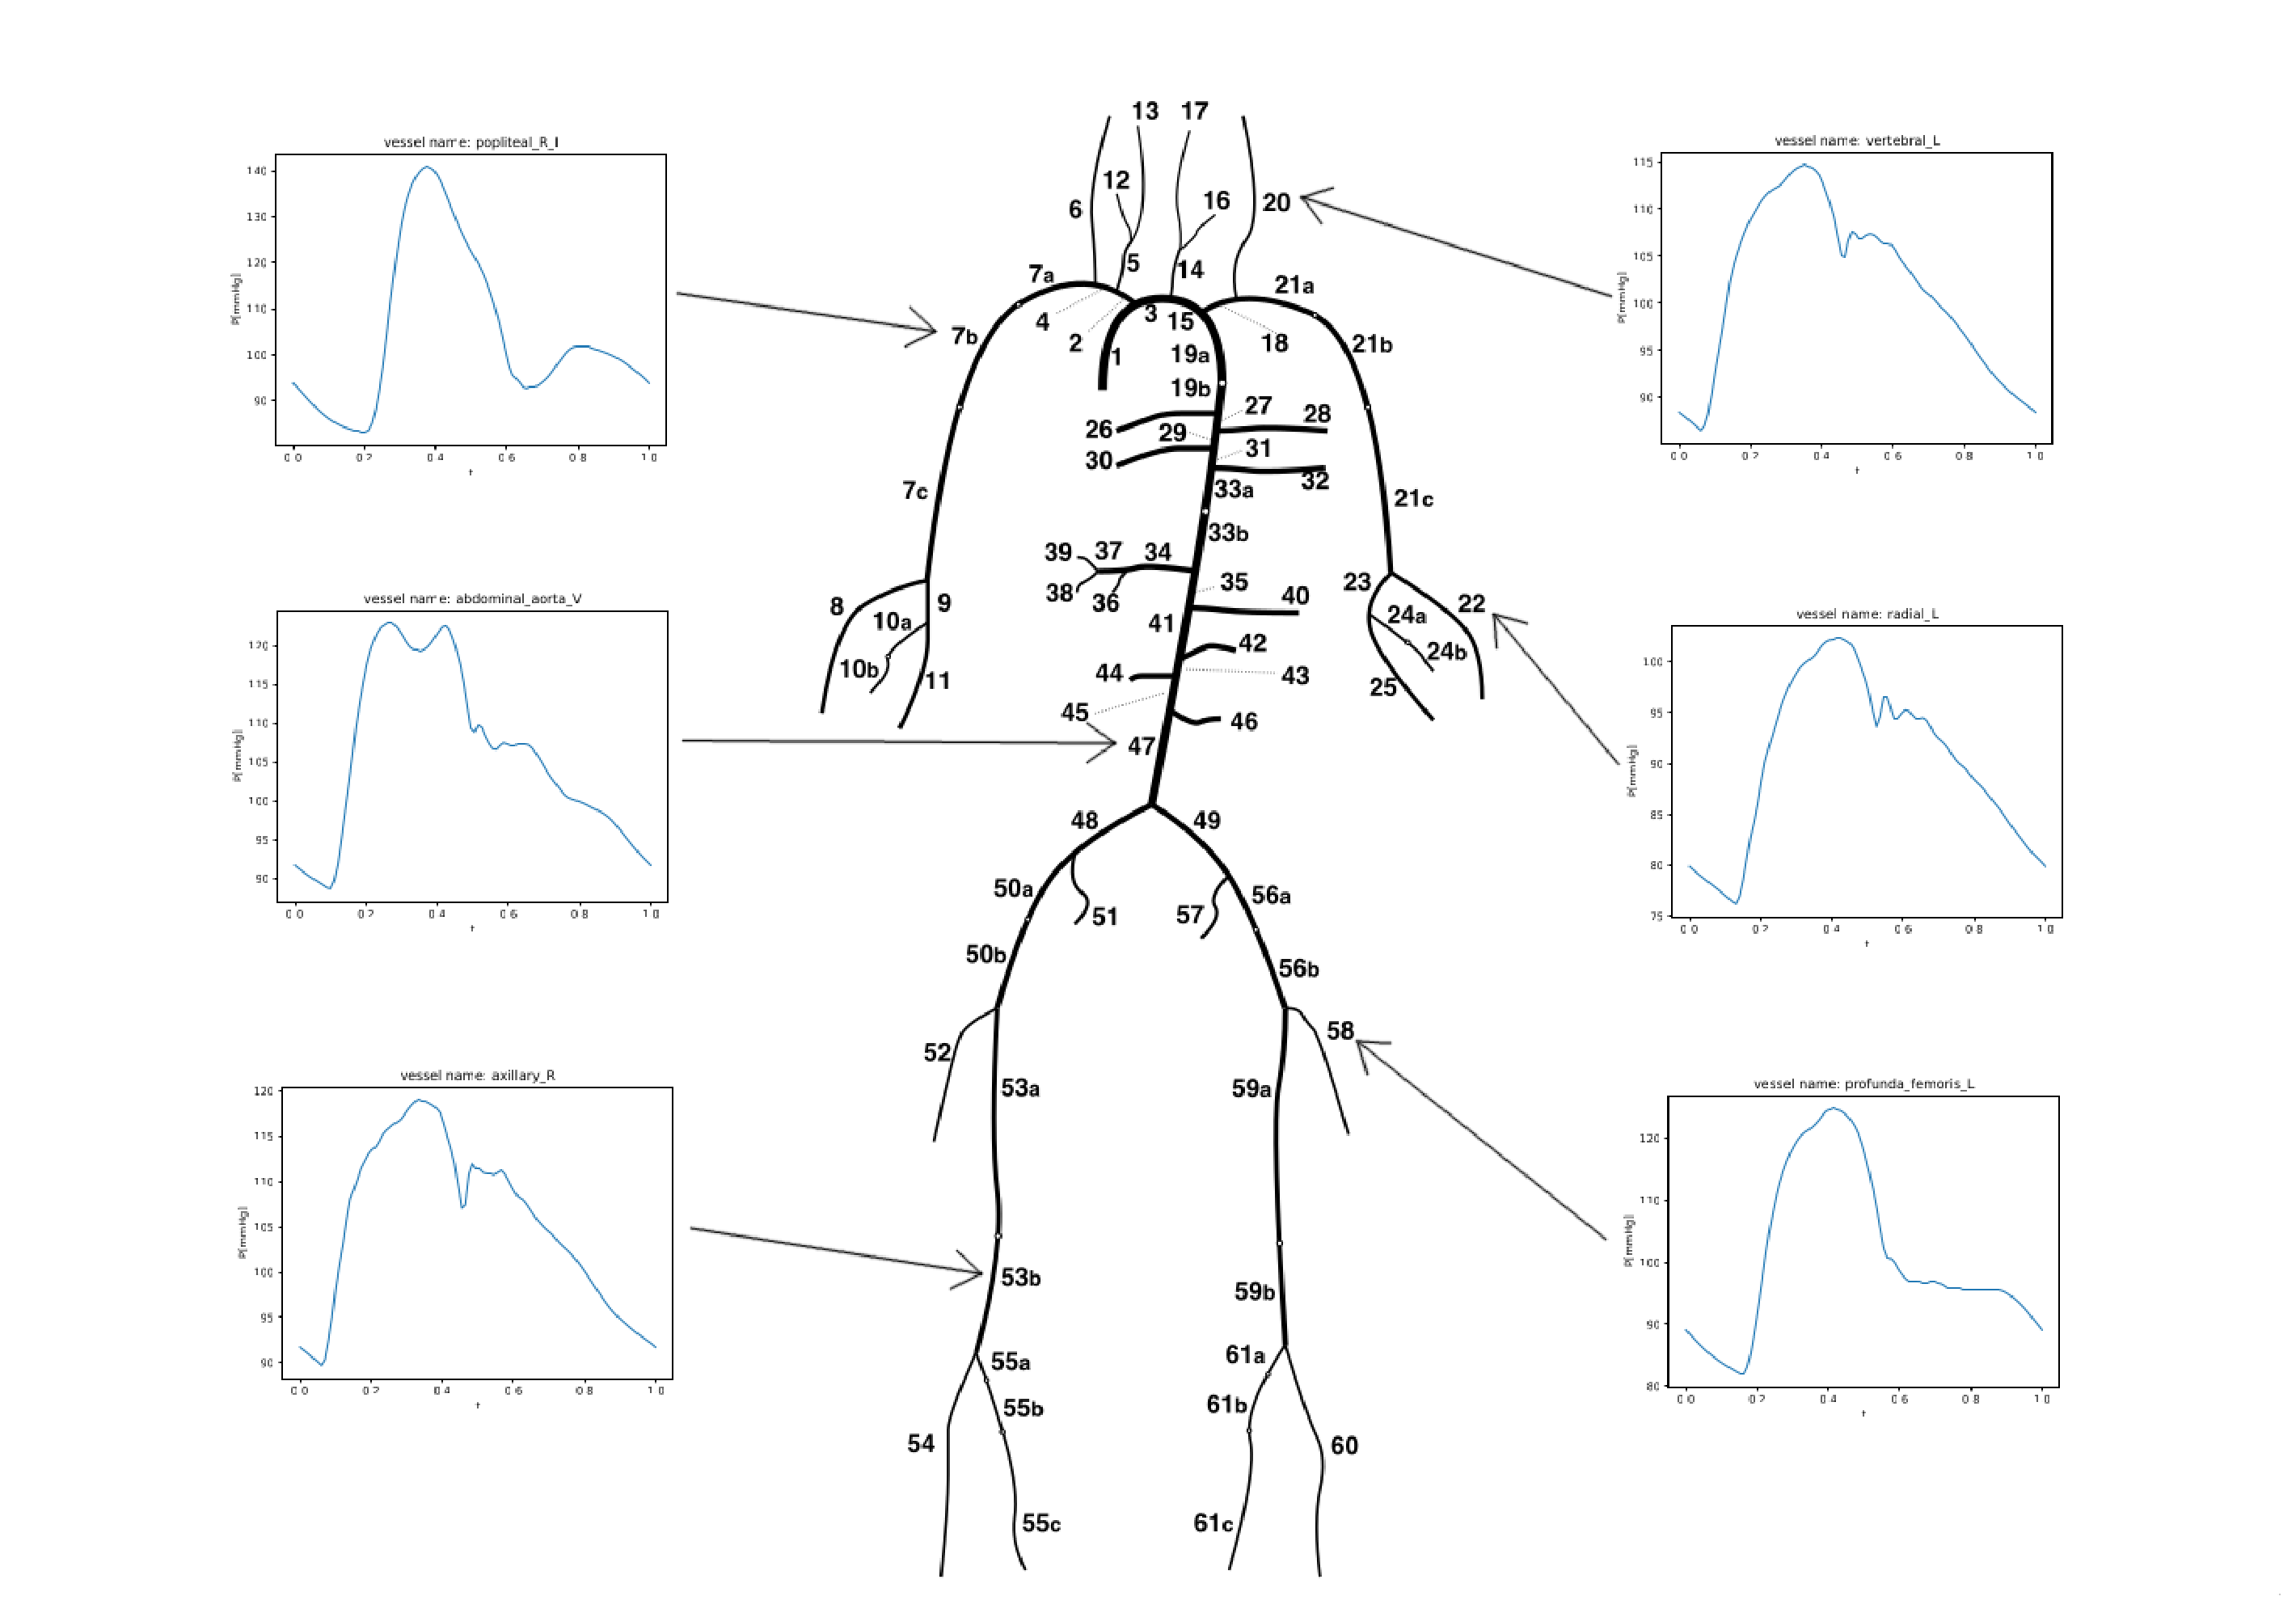
\includegraphics[width=\textwidth]{images/adan56.eps}
\end{frame}
\begin{frame}
	\frametitle{Validation}
	\begin{figure} [H]
		\centering
		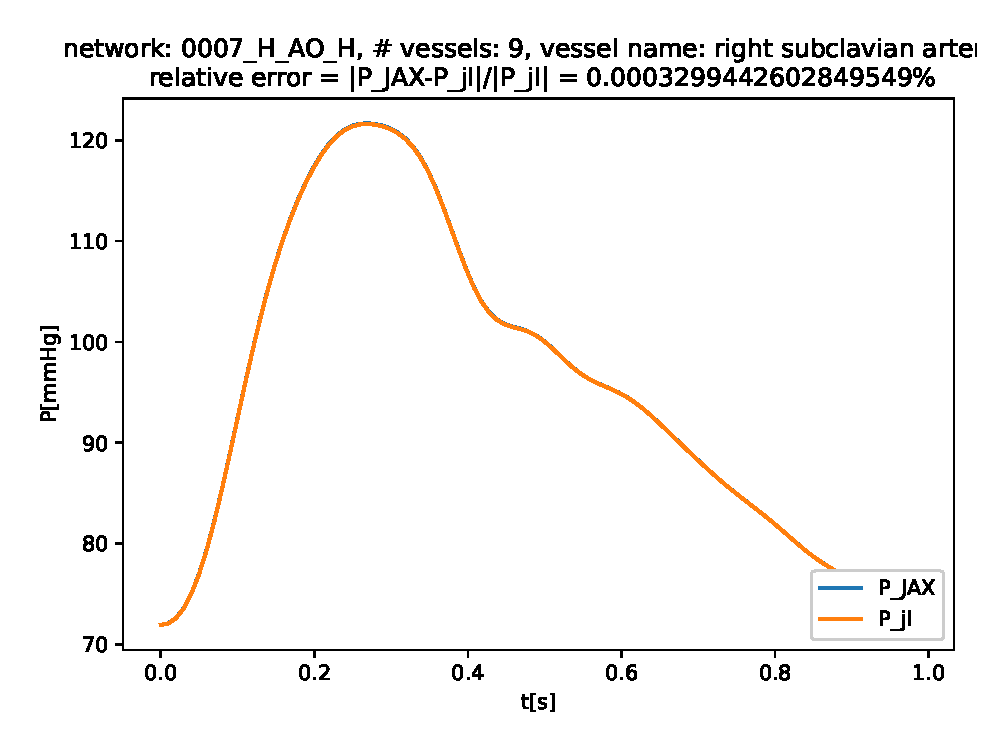
\includegraphics[width=0.46\columnwidth]{images/0007_H_AO_H_right_subclavian_artery_P.eps}
		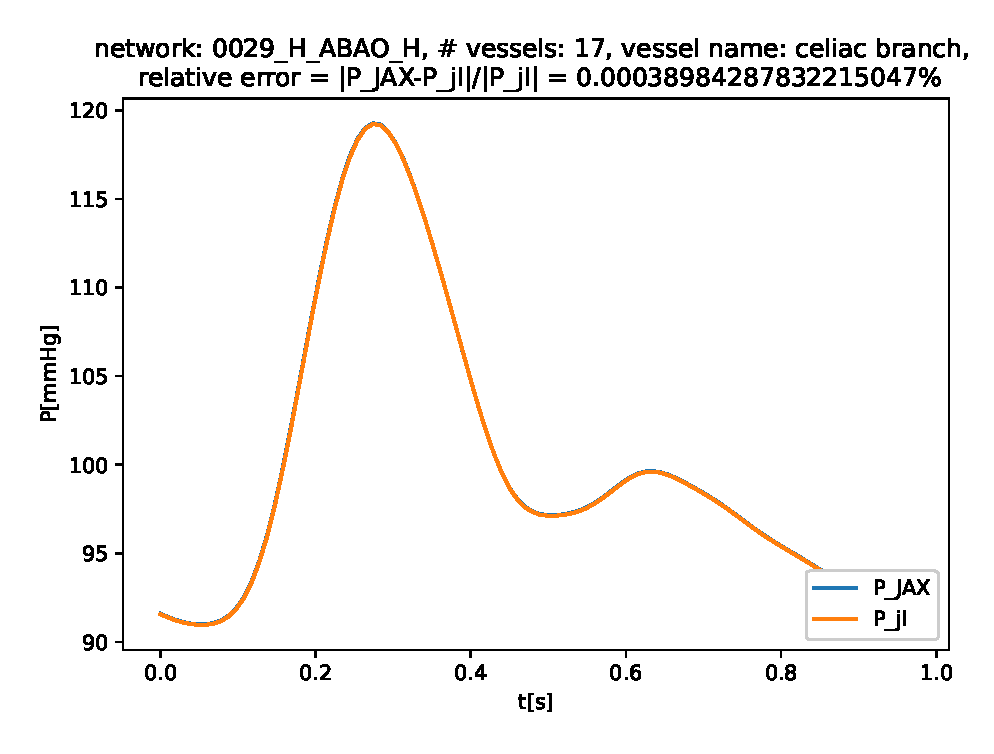
\includegraphics[width=0.46\columnwidth]{images/0029_H_ABAO_H_celiac_branch_P.eps
		}
		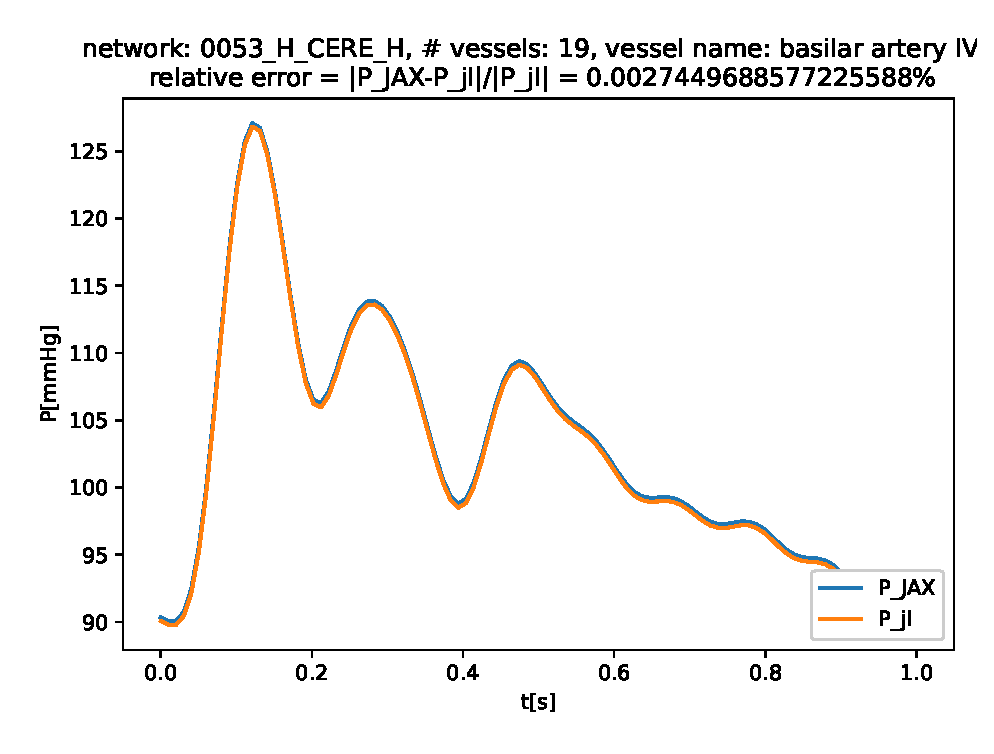
\includegraphics[width=0.46\columnwidth]{images/0053_H_CERE_H_basilar_artery_IV_P.eps}
		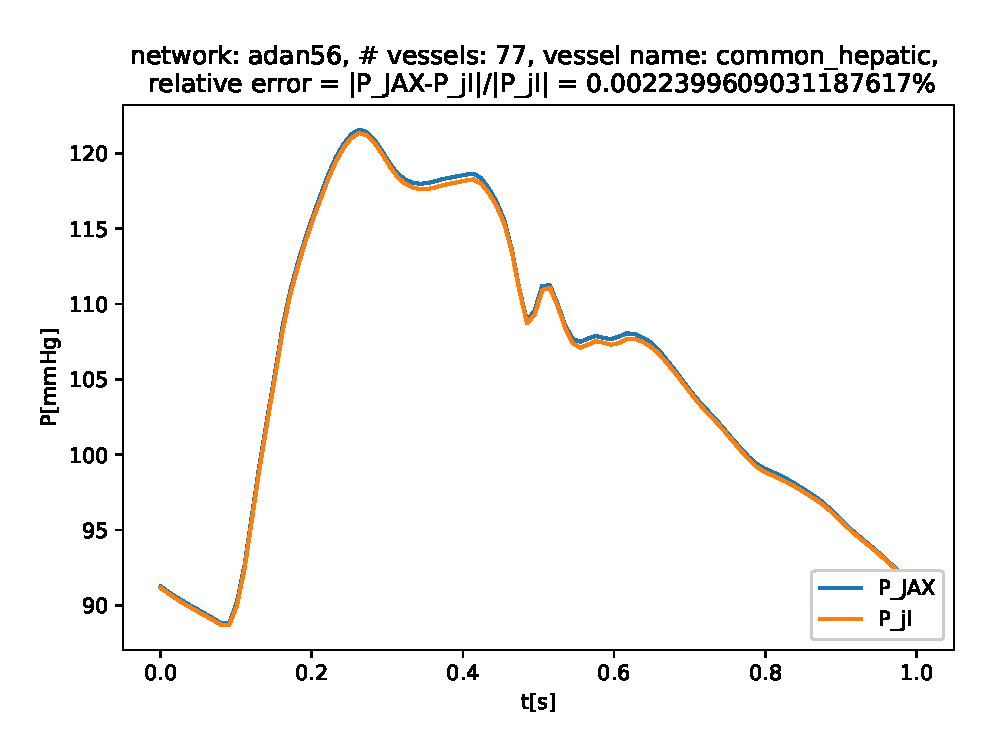
\includegraphics[width=0.46\columnwidth]{images/adan56_common_hepatic_P.eps}
		\label{fig:val}
	\end{figure}
\end{frame}
\begin{frame}
	\frametitle{Comparison}
	\begin{figure} [H]
		\centering
		\includegraphics[width=0.94\columnwidth]{images/comparison.eps}
		\label{fig:comparison}
	\end{figure}

\end{frame}
\begin{frame}
	\frametitle{Inference}
	\begin{block}{Demo}
		inferring an outlet resistance parameter from precomputed data
	\end{block}
\end{frame}

\section{Future Work}
\begin{frame}
	\frametitle{Future Work}
	\begin{block}{Main Points of Interest}
		\begin{itemize}
			\item improving performance (GPU optimization)
			\item fine tuning parameter inference
			\item sensitivity analysis
		\end{itemize}
	\end{block}
	\vspace{5mm}
\end{frame}

\begin{frame}
	\frametitle{Questions?}
	Thank you for your attention!
\end{frame}

\end{document}
